\documentclass[en,license=none]{../../../eplsummary}
\usepackage{framed}
\usepackage{placeins}
\usepackage{listings}
\usepackage{color}
\usepackage{fourier}
\usepackage[]{algorithmicx}

\definecolor{dkgreen}{rgb}{0,0.6,0}
\definecolor{gray}{rgb}{0.5,0.5,0.5}
\definecolor{mauve}{rgb}{0.58,0,0.82}

\DeclareMathOperator{\scp}{scp}
\DeclareMathOperator{\rel}{rel}
\DeclareMathOperator{\sol}{sol}

\lstset{frame=tb,
  language=Java,
  aboveskip=3mm,
  belowskip=3mm,
  showstringspaces=false,
  columns=flexible,
  basicstyle={\scriptsize\ttfamily},
  numbers=none,
  numberstyle=\tiny\color{gray},
  keywordstyle=\color{blue},
  commentstyle=\color{dkgreen},
  stringstyle=\color{mauve},
  breaklines=true,
  breakatwhitespace=true,
  tabsize=3
}

\graphicspath{{res/}}

\hypertitle{Advanced Algorithms for Optimization}{7}{INGI}{2266}
{Houtain Nicolas\and de Vogelaere Cyril\and Gusbin Quentin\and Nicolas Vrielynck}
{Pierre Schaus}

\section{Dynamic programing}H

\subsection{Definition}

\textbf{Dynamic programming} is a method by recurrence in order to solve complex problem.
\begin{itemize}
    \item breaking it down into a collection of simpler subproblems
    \item solving each of those subproblems just once, and storing their solutions in memory
    \item[$\rightarrow$] Next time the same subproblem occurs, instead of 
recomputing its solution, only looks up to the previously computed solution.
Thereby \textbf{saving computation time at the expense of storage space}.
\end{itemize}

\subsection{Solving the knapsack problem with DP}

\subsubsection{The knapsack problem}
\begin{itemize}
    \item A set of item $I$
    \item for each item $i \in I$ is associated a value $v_i$ and a weight $w_i$.

    \item[Goals] 
        \begin{tabular}{m{3cm}m{12cm}}
            $\sum_{i \in I} v_i x_i$: & Maximize the value of selected items\\
            $\sum_{i \in I} w_i x_i \le C$ & Under constraint that the total
            capacity cannot exceed a given maximal capacity $C$ \\ 
            $x_i \in \{0,1\}$ & And an item cannot be partially selected \\
        \end{tabular}
\end{itemize}

Note that Knapsack is an NP-Complete problem as it can be used
to find a solution to the subset-sum problem, which is NP-complete.

\paragraph{Subset-sum problem}

Given a set of natural number and a capacity K. 
Find a subset S such that :
$$\sum_{i \in S} c_i = K$$


\subsubsection{Solutions}
\begin{itemize}
    \item \textbf{DP for knapsack in 0(Cn)}.

        Refer to the optimal objective of the problem with capacity $k$ and
        items \{1,…,j\} $\in$ I as $O(k,j)$. We can easily notice that :

        \begin{itemize}
            \item $O(k,0) = 0 \text{\footnotemark}$
            \item $ O(k,j) = \begin{cases} 
                    max(O(k,j-1) , vj +O(k-wj,j-1))\text{\footnotemark} & if \quad w_j \leq k \\
                    O(k,j-1) & otherwise
                \end{cases}$
        \end{itemize}
        \footnotetext{As their are no elements to choose from}
        \footnotetext{Bellman's equations}


        \begin{lstlisting}[caption=Knapsack DP]
val items = Array((1,1),(6,2),(18,5),(22,6),(28,7)) // (value,weight)
val C = 11
def O(j: Int, k: Int): Int = {
    if (j < 0) 0
    else {
        val (vj,wj) = items(j)
        if (wj > k) O(j-1,k)
        else O(j-1,k).max(vj + O(j-1,k-wj))
    }
}
println(O(items.size-1,C))
        \end{lstlisting}

        \begin{center}
    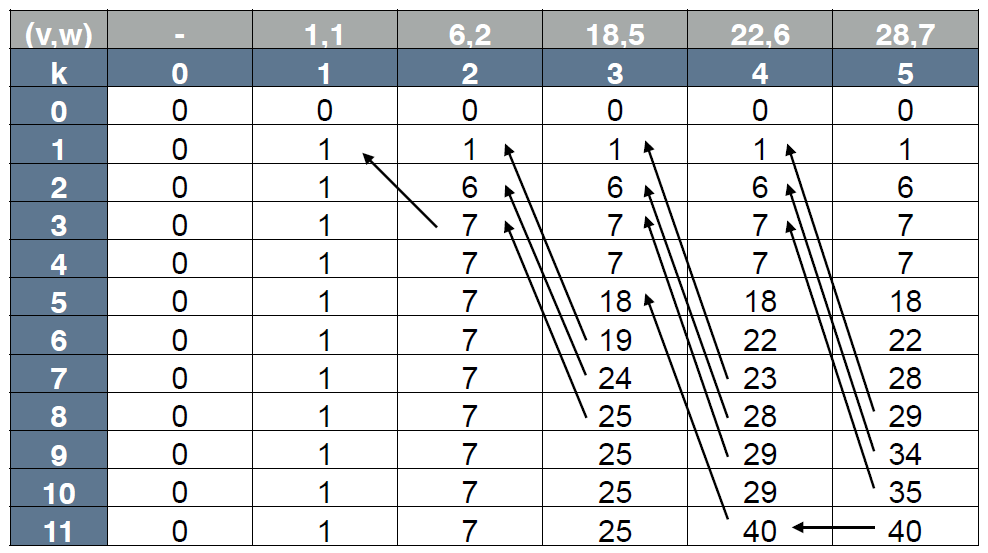
\includegraphics[width=7cm]{KnapsackDP.png}
        \end{center}

    \item \textbf{DP for knapsack in 0(Vn)}.

        Using a similar logic, it is also possible to define an algorithm which
        run in $\theta$(Vn) to compute knapsacks. Let $V = \sum_{i \in I} v_i$,
        we can redefine O(k,j) as O(w,j), the optimal weight using only items
        \{1,...,j\}. The equation will thus change as follow :

    \begin{itemize}
    \item $O(0,j) = O(p,0) = 0 \text{\footnotemark} $
    \item $ O(p,j) = \begin{cases}
                min(O(p,j-1), wi + O(p-v_j,j-1)) & if \quad v_j \leq p \\
                O(p,j-1) & otherwise
            \end{cases}$
        \end{itemize}
        \footnotetext{As $w_i > 0$ for all $i \in I$ and as we cannot have w > 0 with 
        an empty set.}
        \begin{center}
            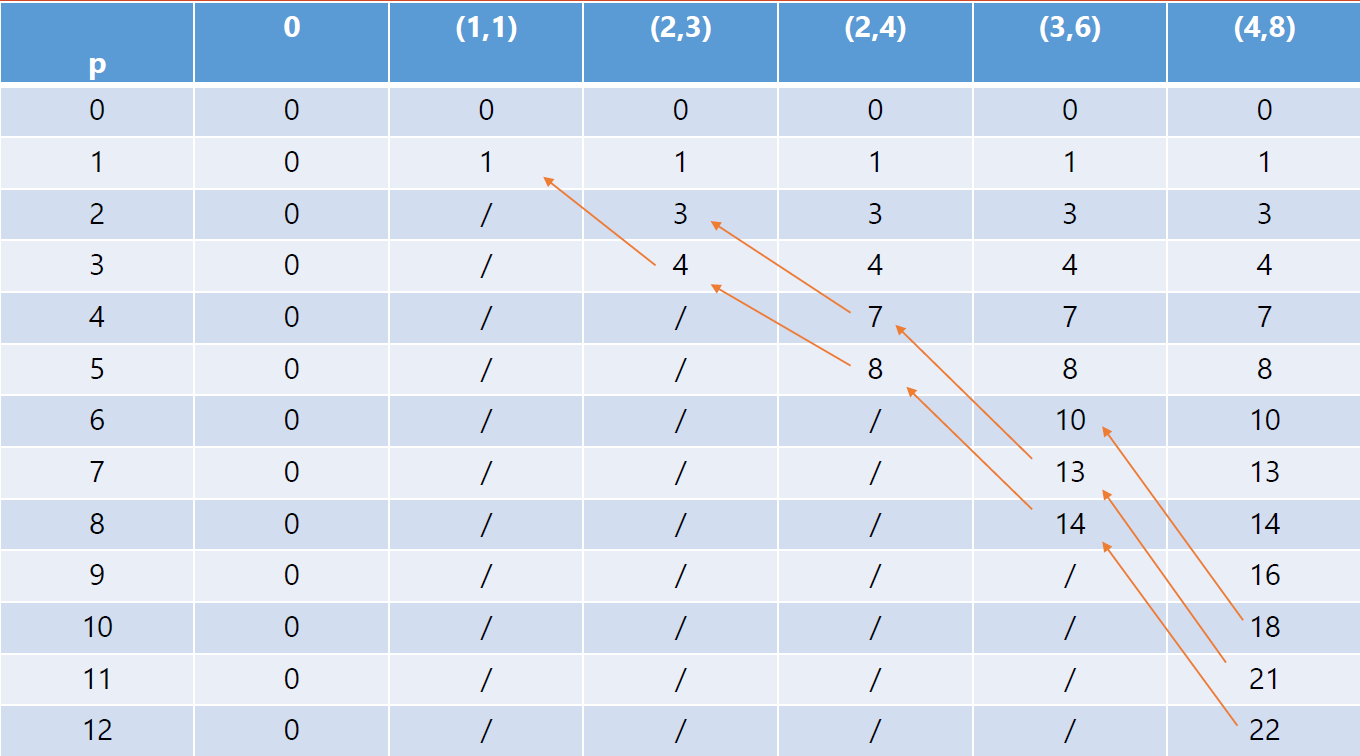
\includegraphics[width=7cm]{KnapsackDPAlgo2.png}
        \end{center}
\end{itemize}

\subsubsection{Cache usage}
\begin{tabular}{m{9cm}m{6cm}}
As explain, a cache is use in order to store computed value and avoid to recompute
it. In \textcolor{red}{red} we have the cells actually computed.
&
    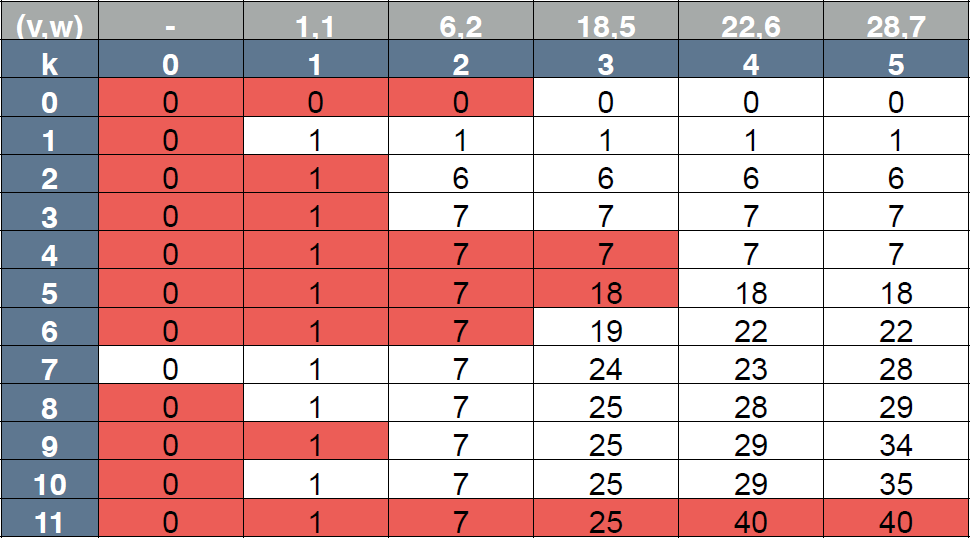
\includegraphics[width=6cm]{KnapsackDPAlgo1.png}
\end{tabular}


\subsubsection{Pseudo-polynomial}

DP is \textsc{pseudo-polynomial}, since it is exponential in the 
\textit{length of input} ($log(C)$) which is the number of bits required to
encode the input ($C$). The complexity is thus exponential relatively to the
input size. This algorithm is \textbf{weakly NP-Complete} or
\textbf{pseudo-polynomial}\footnote{a numeric algorithm runs in
pseudo-polynomial time if its running time is polynomial in the numeric value
of the input, but is exponential in the length of the input – the number of
bits required to represent it.} as it is roughly polynomial for small values of
C while computing larger value is much more expensive\footnote{Not all
    NP-Complete algorithm are pseudo polynomial ! Like the traveling salesman
problem (TSP), for example.}.


\subsection{Other examples of DP algorithms}

Before reading this section, please remember that all algorithm that can be
implemented via dynamic programming are not ipso-facto pseudo polynomial ! Any
algorithm can be expressed with dynamic programming as long as it can be separated in
sub problems.

%\subsubsection{TSP}
%Say $1$ be the source of the TSP.
%\begin{itemize}
%    \item $O(S,1) = 0 $
%    \item $ O(S, j) = 
%        min\Bigg( \{ \quad O\bigg(S -\{j\}, i\bigg) + d_{ij} \quad
%            |\quad  i \in S \wedge i \in
%        Neighboor(j)\quad \} \Bigg)$
%\end{itemize}
%
%The answer to join $1$ to $n$ is $O(AllVertex, n)$


\subsection{Exam}
I give you a problem (for instance the TSP, Knapsack)
\begin{itemize}
    \item  Design a greedy algorithm
    \item  Design a Dynamic Programming formulation
    \item  Design a relaxation and upper/lower bound
        procedure and embed it in a Branch and Bound
    \item  Justify advantages and disadvantages of each
    \item  Apply the three techniques to a small instance
        manually
\end{itemize}


\section{Branch and bound}

\subsection{Definition}

A \textbf{branch-and-bound} algorithm consists of a systematic enumeration of
candidate solutions by means of state space search: the set of candidate
solutions is thought of as forming a rooted tree with the full set at the root.

\begin{itemize}
    \item Explores branches of this tree, which represent subsets of the
solution set. 
    \item Note that before enumerating the candidate solutions of a branch, the
branch is checked against upper and lower estimated bounds on the optimal
solution, and is discarded if it cannot produce a better solution than the best
one found so far by the algorithm.
\end{itemize}

\subsection{Solving the knapsack problem with B\&B}

Given the following knapsack problem :
    \begin{tabular}{cl}
        maximize & $28x_1+30x_2 +20x_3$\\
        subject to & $4x_1+6x_2 +4x_3 \leq 9$\\
                   & $x_i \in \{0, 1\} \forall i$
    \end{tabular}

\subsubsection{Relaxation}
We can choose to relax in order to reduce the search space as much as possible.

\begin{enumerate}
    \item \textbf{Capacity relaxation}: Relax on the constraint by don't
        explore branch which already violated the constraint.

        $\Rightarrow$ Cut at tree branch when 
        we have surpassed the capacity.
        \begin{center}
        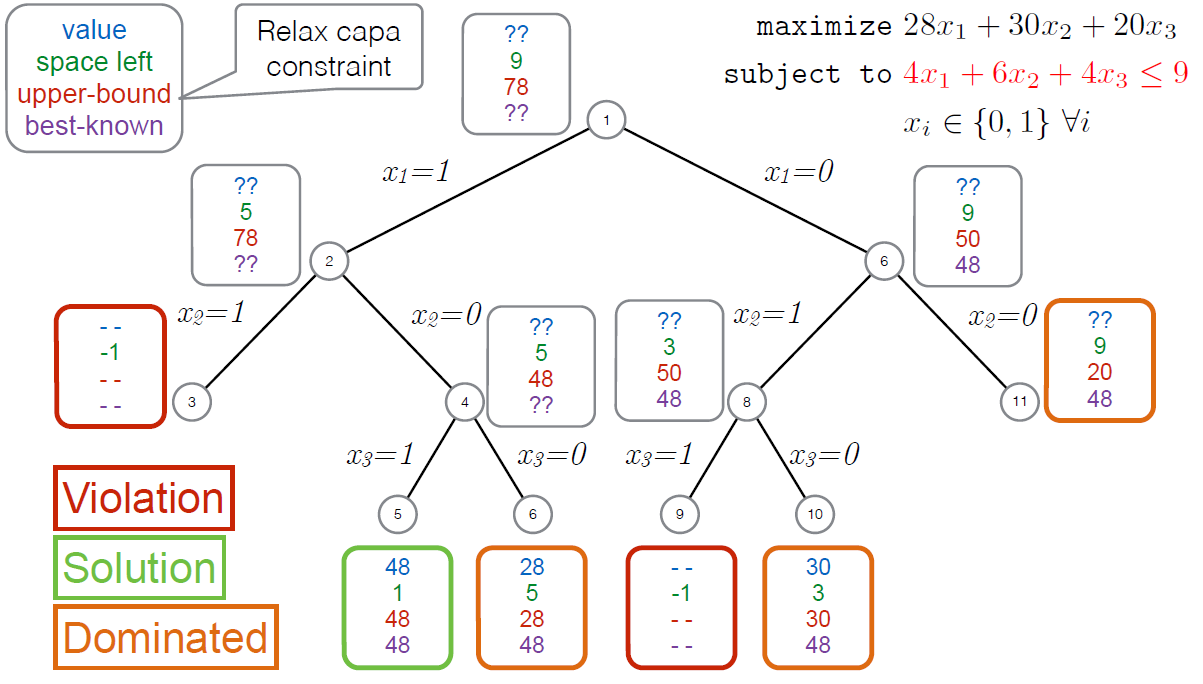
\includegraphics[width=12cm]{KnapsackBBCapaRelaxation.png}
        \end{center}
        It is far from optimal as our upper bound are not close enough to their real
        value.

    \item \textbf{Linear relaxation}: Relax on the value to maximize by
        calculating an upper bound and don't explore if the upper bound <
        actual best value.

        \paragraph{Upper bound computation}
        Given a set sorted by ratio $v_i/w_i$,
        \begin{eqnarray*}
            j &= min\{i \in I: \sum_{k \in 1,...,i} w_k > C\}\\
            UB &= \sum_{i<j} v_i + \frac{(C - \sum_{i \in 1..j-1} w_i)}{w_j} v_j
        \end{eqnarray*}

        $j$ is called the critical item which is in fact the first item (sorted by better ratio)
        which cannot be add entirely, so we just add the ratio of the item according to 
        the free space.

        \begin{center}
            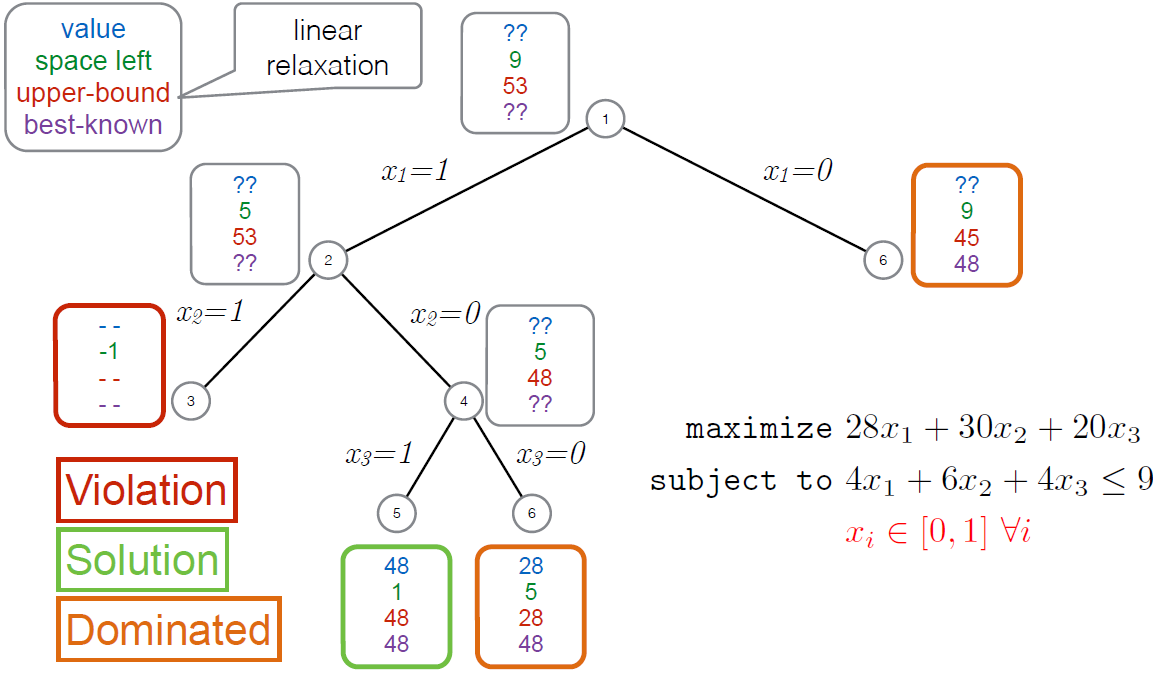
\includegraphics[width=12cm]{KnapsackBBLinearRelaxation.png}
        \end{center}

        Improving the precision of the upper-bound yields far better
        result. Take care however not to over/under estimate it (depending if you are
        on a maximisation or minimisation process) as it might prevent you to find the
        optimal solution.

\end{enumerate}


\subsection{B\&B pseudo-code}

\begin{tabular}{m{8cm}m{8cm}}
\begin{lstlisting}[mathescape, caption=BB with recursion]
def backtrackSearch(c) {
    if reject(P, c) then return
    if accept(P, c) then output(P, c)
    for s $\leftarrow$ children(c) do
        backtrackSearch(s)
}

backtrackSearch(root(P))
\end{lstlisting}
&
\begin{lstlisting}[mathescape, caption=BB with stack]
  def branchAndBound() = {
      var queue = List(root(P))

      while(queue.nonEmpty) {
          var c = queue.head
          queue = queue.tail

          if( ! reject(P, c)) {
            if( accept(P, c)) output(P, c)
            for (s $\leftarrow$ children(P, c))
            queue = s :: queue
          }
      }
  }
  \end{lstlisting}
\end{tabular}


\begin{itemize}
    \item For the knapsack, partial solution by a list of boolean: 
        $\begin{cases} 
            list[i]= 1 \text{ if item i is selected}\\
            list[i]= 0 \text{ else}\\
        \end{cases}$
\end{itemize}

\begin{center}
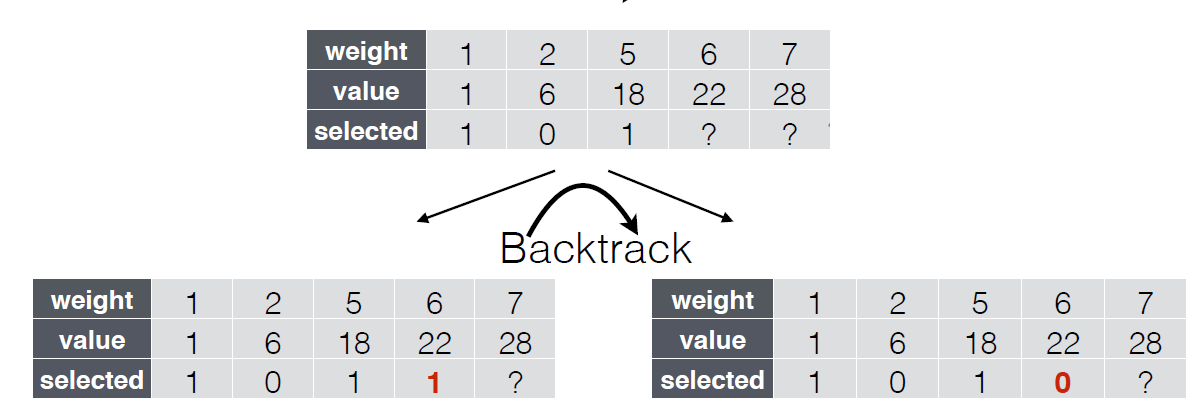
\includegraphics[width=10cm]{PartialSolBB.png}
\end{center}

\paragraph{Limitations which may affect performance}:
\begin{itemize}
    \item Must evaluate variable in the same order. We cannot affect $X_1$
        then$ X_2$ at the left side of the tree while on the other side we
        affect $X_2$ then $X_1$, each level of the tree must strictly
        correspond to the affectation of a variable.

    \item Cannot process trees which has a variable number of children easily.
        If it's the case, we could, for example, decide multiple variables at once.
\end{itemize}

\subsection{Reversible state and magical integers}

\textbf{Reversible states} are use to improve our algorithm in two way:
\begin{enumerate}
    \item By breaking the two previous limitation
    \item By use only one incremental state relative of the change
        that have been made on the parent instead of
            simply clone the parent and waste memory.
\end{enumerate}
        
\subsubsection{The idea}

To implement those reversible states, we will thus make use of three objects.

\begin{enumerate}
	\item \textbf{ReversibleContext()} : Which will be used to represent a 
	reversible state.
	\item \textbf{ReversibleInt(ReversibleContext rc, int i)} : Which will be used to 
	represent the variables of a reversible state.
	\item \textbf{TrailEntry(ReversibleInt ri, int value)} : Which will be used
	to represent changes on a stacks stocked in the context. This object will
	only be used by the ReversibleContext class.
\end{enumerate}

\begin{tabular}{m{8cm}m{7cm}}
\begin{lstlisting}[mathescape]
val rc = new ReversibleContext() 
val n1 = new ReversibleInt(rc,2)
val n2 = new ReversibleInt(rc,5) 

rc.pushState()    // Store $n_1=2$ and $n2=5$

n1.value = 6
n1.value = 5
n2.value = 4

rc.pushState()    // Store $n_1=5$ and $n2=4$

n1.value = 3
n2.value = 7

rc.pop()          // Restore $n_1=5$ and $n_2=4$
rc.pop()          // Restore $n_1=2$ and $n_2=5$
\end{lstlisting}
& 
\begin{itemize}
    \item Each reversible contains the \textbf{time} at which its last value was given
    \item A each \texttt{pushState()} the clock increase
    \item When the value of a reversible change, if its last value was given at a
        time different from the current time, then we store it before actually changing
        the current value
    \end{itemize}
\end{tabular}


\subsubsection{Push/Pop operation in reversible context}
\begin{center}
    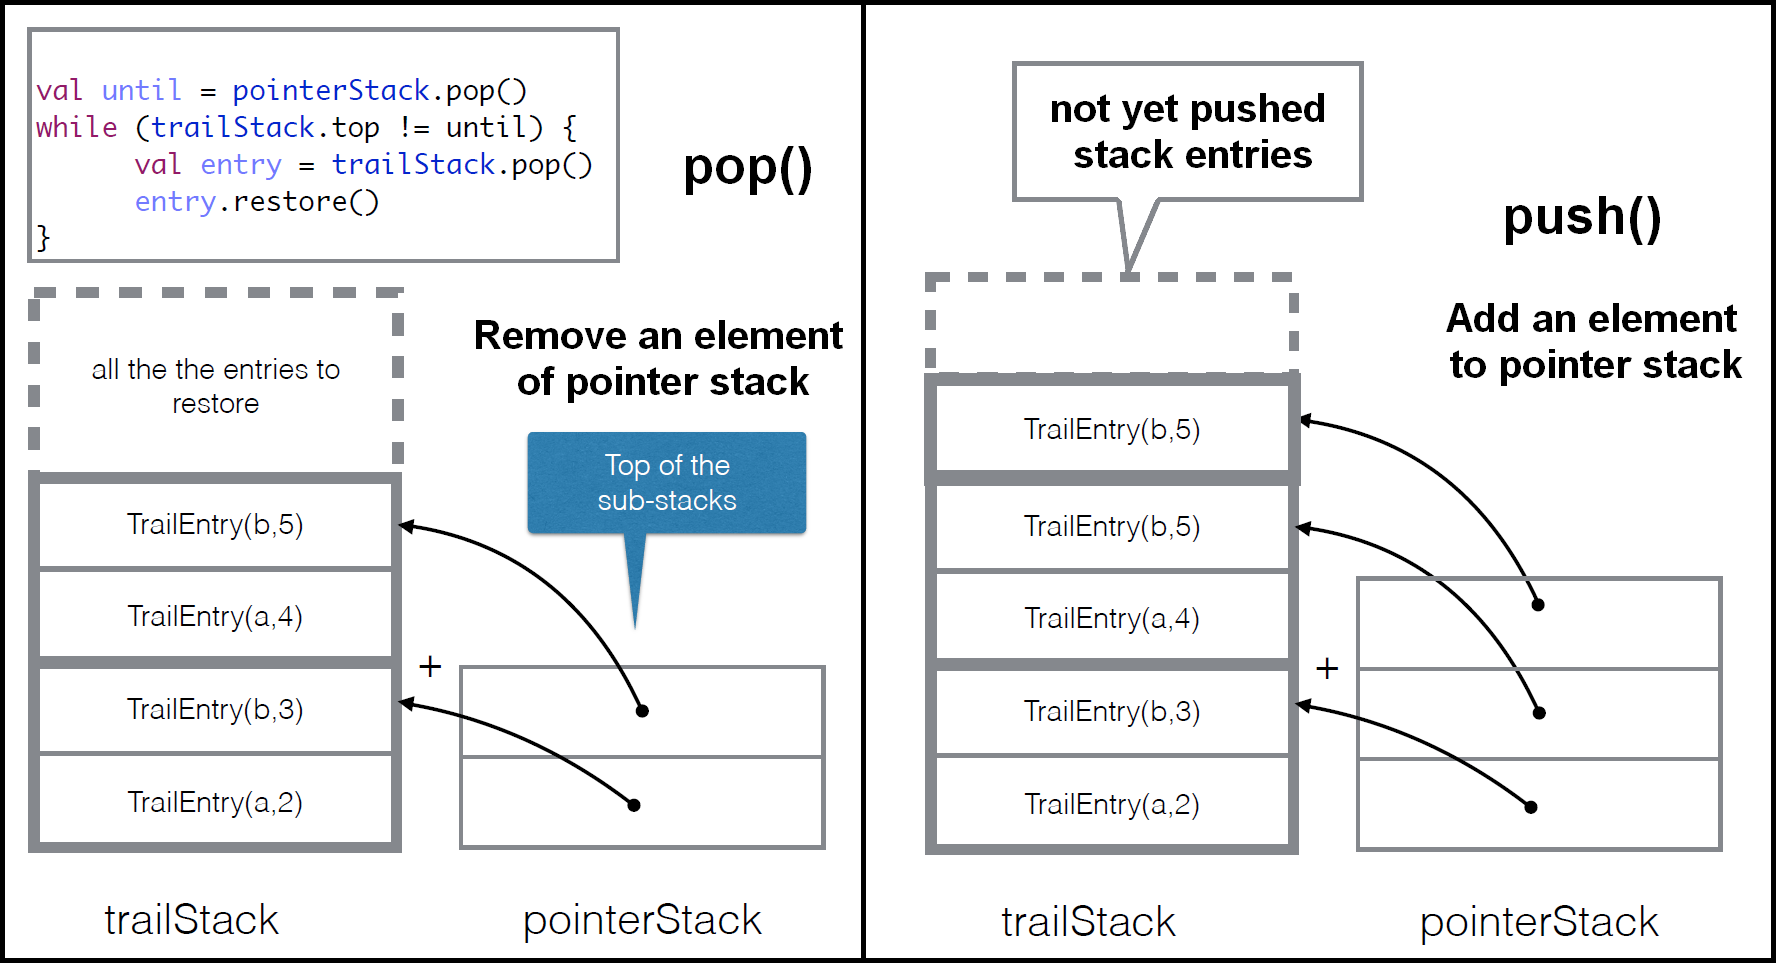
\includegraphics[width=12cm]{ReversibleStatePushPop.png}
\end{center}

\subsubsection{Implementation}

\begin{tabular}{m{8cm}m{7cm}}
\begin{lstlisting}[mathescape]
class ReversibleContext() {
    private var magicNumber: Long = 0
    private val trailStack: Stack[TrailEntry] = new Stack()
    private val pointerStack: Stack[TrailEntry] = new Stack()

    def magic: Long = magicNumber
    def pushOnTrail[T](reversible: ReversibleInt, value: Int): Unit = {
        val entry = new TrailEntry(reversible, value)
        trailStack.push(entry)
    }
    def pushState(): Unit = {
        magicNumber += 1
        pointerStack.push(trailStack.top)
    }
    def pop(): Unit = {
        restoreUntil(pointerStack.pop())
        magicNumber += 1
    }
    def restoreUntil(until: TrailEntry): Unit = {
        while (trailStack.top != until) {
            val entry = trailStack.pop()
            entry.restore()
        }
    }
}
\end{lstlisting}
& 
\begin{lstlisting}[mathescape]
class ReversibleInt(context: ReversibleContext, v: Int) {
    protected var pointer: Int = v
    private var lastMagic: Long = -1L
    trail()

    def trail(): Unit = {
        val contextMagic = context.magic
        if (lastMagic != contextMagic) {
            // Store previous value on store 
            // because magic time has changed
            lastMagic = contextMagic
            context.pushOnTrail(this, value)
        }
    }
    def value_=(value: Int): Unit = {
        if (value != pointer) {
            // Before overriding, trail it if necessary
            trail()
            this.pointer = value
        }
    }
    def value = pointer
    def restore(value: Int): Unit = pointer = value
}
\end{lstlisting}
\end{tabular}

\paragraph{Implementation B\&B using reversible}
Show example lecture 2 page 28

\subsection{Search heuristics}
With heuristic, we can at each given moment, decide what variable to instantiate 
and/or which value to assign. 

\begin{itemize}
    \item Variables heuristic: Choose which variable will know be 
        assigned
    \item Value heuristic: Choose the order of assigned value for
        the variables
    \end{itemize}

\subsubsection{Iterative Discrepancy Search}

\begin{tabular}{m{11cm}m{6cm}}
\begin{description}
    \item[Discrepancy] = Number of right (the side in a tree) decisions
\end{description}
\begin{lstlisting}[mathescape]
for (d $\leftarrow$ 0 to 100) {
    problem.search(maxDiscrepancy = d)
}
\end{lstlisting}
&
    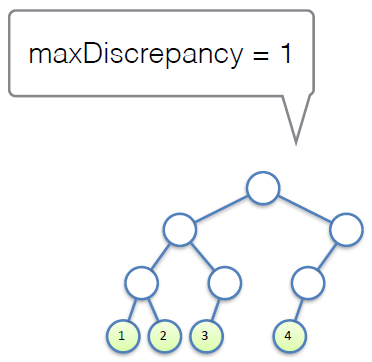
\includegraphics[width=4cm]{LimiteDiscrpancy.png}
\end{tabular}


\paragraph{Advantages}
\begin{itemize}
    \item Easy to implement, weak memory consumption (DFS)
    \item Can potentially be fast \textbf{depending on the heuristics},
        but also slower because of recomputation which are normally for the
        most part pruning in recomputation.
\end{itemize}

\textbf{If the discrepancy search does not explore the tree completely, 
it is not considered complete !} This can however be used as a form of greedy
algorithm.

\subsubsection{Best first search}

Expand the open node with the best upper-bound first (maximization) !
Although fairly efficient and easy to implement, this heuristic has two drawbacks :

\begin{enumerate}
	\item You won't have a feasible solution directly (implication for the pruning).
	\item Memory usage is difficult to control.
\end{enumerate}

\begin{figure}[!ht]
    \centering
    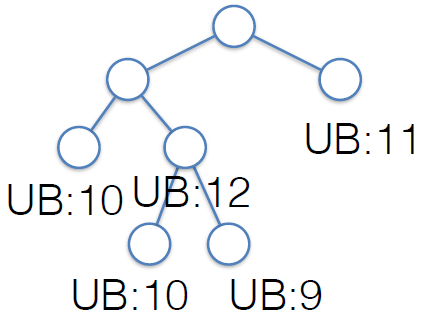
\includegraphics[width=0.3\linewidth]{BestFirstSearchBBHeuristic.png}
    \caption{Representation of the best first search heuristic}
    \label{fig:Knapsack_example}
\end{figure}
\FloatBarrier

\subsubsection{Other heuristics}

TODO

\subsection{Other B\&B optimisations}

\subsubsection{Symmetry detection}

In case of symmetric items in the knapsack set (understand identical), we can reduce the
search space significantly as the items are completely interchangeable.

\subsubsection{Dominance detection}

In case an item b is dominated by another item a
(b is dominated by a if $V_a \geq V_b \wedge W_a \leq W_b$)
It is never interesting to take b if a is not also taken ! 

$\Rightarrow$ An optimal solution cannot have a = 0 and b = 1. 
We can thus avoid to explore such states.

\subsection{Bonus questions}

\subsubsection{Reversible set}

\begin{lstlisting}
//WARNING : UNTESTED but the idea is there

//Create ReversibleSet class as follows
// 1 : Add set variable which store curent set
// 2 : Modify pointer to save multiples changes
// 3 : Add remove method which remove in set and adds to changes made
// 4 : Modify trail method to push changes one by one
// 5 : Modifify restore methode to remove unpushed changes and add back argument value
// 6 : Write the get iterator method

class ReversibleSet(context: ReversibleContext, s: Set) {
	protected var currentSet: Set = s //Set
	protected var pointer: Array<Integer> = [] //List of changes
	private var lastMagic: Long = -1L
	trail()
	
	def trail(): Unit = {
		val contextMagic = context.magic
		if (lastMagic != contextMagic) {
			//We need to push values
			lastMagic = contextMagic
			for elem in pointer{ //One push per elem removed
				context.pushOnTrail(this, elem)
			}
			pointer = [] //Reset change array since change have been pushed
		}
	}
	def remove(value: Int): Unit = {
		if (value != pointer) {
			trail() //Always call this method before making changes
			this.currentSet.remove(value) //Remove value in set
			this.pointer.add(value) //Add to changes made
		}
	}
	def getIterator() : Unit = {
		return set.iterator(); //Assuming our set implements iterable
	}
	def set = currentSet //To acces current set value
	
	def restore(value: Int): Unit = {
		//Remove unpushed changes
		for elem in value{
			set.add(elem)
		}
		//(so that we don't add multiple time in case of multiple changes)
		pointer = [] //Reinit change list 
		//Add the value in argument to the set
		set.add(value);
	}
}
\end{lstlisting}

\subsubsection{Explicit stack DFS's pseudo code}

\begin{lstlisting}
//Init stack
stack state_to_visit = new stack();
state_to_visit.add((0,initState)); 
//A tuple (current index, state where no item are taken)
//Init method variable
int maxIndex = nbVariableToAsssign - 1;
state bestSol = initState;
while(!state_to_visit.isEmpty()) {
  (index, state) = state_to_visit.pop();
  if(index > maxIndex){
  	//Computation finished, evaluate state
  	if(bestSol.value < state.value) bestSol = state;
  }
  else if(state.getUpperBound() > bestSol.value){
  	newState = state.makeCopy()
  	//Add current elem not selected state to stack
  	state_to_visit.push((index+1, state));
  	//Add current elem selected state to stack => will be visited first
  	newState.changeElemAtIndex(index, 1); //Set as taken
  	if(newState.isUnderCapacityConstraint()) state_to_visit.push((index+1, newState));
  }
}
return bestSol; 
\end{lstlisting}

\subsection{Exam}
\begin{itemize}
    \item Give the pseudo-code of a backtracking search algorithm
        \begin{itemize}
            \item  What kind of search tree exploration is it?
            \item  What are the advantages of such an exploration?
        \end{itemize}
    \item Explain the trailing and reversible mechanism
        \begin{itemize}
            \item  Sketch the code to implement it, give an example of how to use
                it
            \item  Illustrate the solving of a combinatorial problem with a
                backtracking search using reversibles to restore state
        \end{itemize}
    \item  Explain Limited Discrepancy Search, why it is useful? How to
        implement it using DFS while staying complete
    \item  Explain/Illustrate the heuristics and how it can impact B\&B
    \item  Explain what are symmetries and dominances, how to avoid
        them?
\end{itemize}


\section{Linear programming}
\subsection{Definition}

Linear programming consist of a maximisation of a linear fonction subject to linear constraints.

\subsubsection{Example}

\begin{tabular}{m{8cm}m{5cm}}
    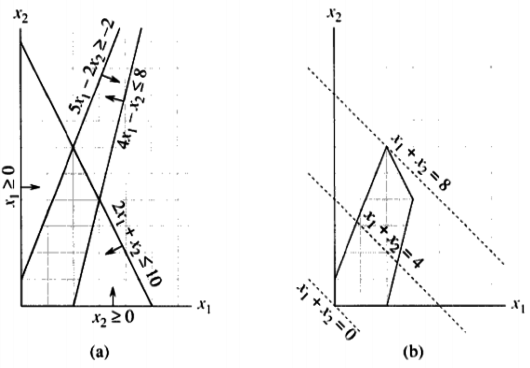
\includegraphics[width=7cm]{example1.png}
    &
    \begin{eqnarray*}
        \textrm{maximize } & x_1 + x_2 \\
        \textrm{subject to } & 4x_1 - x_2 & \leq 8 \\
                             & 2x_1 + x_2 & \leq 10 \\
                             & 5x_1 - 2x_2 & \geq -2\\
                            & x_1, x_2 \geq 0
        \end{eqnarray*}
\end{tabular}

\subsection{Polytope}

The solution space is a \textbf{polytope}. In a polytope, every point is a convex
combination of its vertices:
$$(\alpha x + (1 - \alpha)y) \in S \, \quad  with \quad \, \alpha \in
[0,1]$$

\begin{tabular}{m{8cm}m{4cm}}
    \begin{eqnarray*}
        \textrm{maximize } & c_1x_1 + ... + c_nx_n \\
        \textrm{subject to } & a_{11}x_1 + ... + a_{1n}x_n \leq b_1 \\
                             & ... \\
                             & a_{m1}x_1 + ... + a_{mn}x_n \leq b_m \\
        \end{eqnarray*}
        &
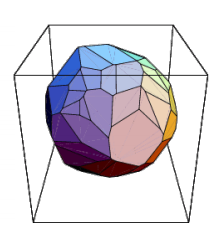
\includegraphics[width=3cm]{polytope.png}
\end{tabular}


\subsubsection{Theorem}
At least one of the points where the objective value is maximal is a vertex of the polytope.
\paragraph{Proof} : 
\begin{itemize}
    \item The maximum $x^{*}$ as a combination of the vertices of the
        polytope $v_{1},...,v_{t}$)
        $$x^{*} = \lambda_{1} v_{1} + ... + \lambda_{t} v_{t}$$

    \item Objective value at optimality can be expressed as a scalar
        product with $c$ a vector
        and the objective value at optimality can be expressed as a scalar product (c is a vector)
        $$c x^{*} = \lambda_{1} * (cv_{1}) + ... + \lambda_{t} * (cv_{t})$$
\end{itemize}

Let's assume that the maximum is not a vertex (each vertex is less good than $x^{*}$) \\
$$cx^{*} > cv_{i} \quad \forall i : 1 \leq i \leq t$$
Then we have 
\begin{align*}
cx^{*} =& \, \lambda_{1} * (cv_{1}) + ... + \lambda_{t} * (cv_{t}) \\
<& \, \lambda_{1} * (cx^{*}) + ... + \lambda_{t} * (cx^{*}) \\
<& \, (\lambda_{1} + ... + \lambda_{t}) (cx^{*}) \\
<& \, cx^{*}
\end{align*}

$\Rightarrow $ With this contradiction we can see that the maximal
$x^{*}$ must be a vertex.

\subsubsection{Algorithm}
We know that the best solution is located on a vertex of the
polytope:
\begin{enumerate}

    \item A naive approach would be to enumerate every vertices and take
        the one with the larget value. But, the problem is that the
        number of vertice grow exponentially with the number of
        inequality. 

    \item A better approach is the simplex algorithm. The idea is to
        move from one vertex to another with an improving objective
        function. We know this to be optimal thanks to the convexity of
        the polytope.
\end{enumerate}

\subsection{Simplex Algorithm}

\subsubsection{Standard and slack forms}
In order to use the simplex algorithm we need 
\begin{enumerate}
    \item Transform our linear problem  to  a \textbf{standard form}
        \begin{enumerate} 
            \item Replace equality to inequality
            \item If variable $x_j$ has no non-negativity
                constraint replace
                each occurrence by $x_j - x_k$
        \end{enumerate}
\begin{scriptsize}
        \begin{tabular}{m{7cm}cm{7cm}}
            \begin{eqnarray*}
                \textrm{maximize } & 2x_1 - 3x_2\\
                \textrm{subject to } & x_1 + x_2 &= 7\\
                                     & x_1 - 2x_2 &\leq 4 \\
                                     & x_1 &\geq 0\\
            \end{eqnarray*}
            & $\Rightarrow$ &
            \begin{eqnarray*}
                \textrm{maximize } & 2x_1 - 3x_2 + 3x_3\\
                \textrm{subject to } & x_1 + x_2 - x_3 & \leq 7\\
                                     & -x_1 - x_2 + x_3 & \leq -7  \\
                                     & x_1 - 2x_2 + 2x_3 & \leqq 4 \\
                                     & x_1, x_2, x_3 & \geq 0\\
            \end{eqnarray*}
        \end{tabular}
\end{scriptsize}

    \item then transform standard form to a \textbf{slack form }.
        $\Rightarrow$  Introduction of basis variable in order to find a 
        \textbf{Basic Feasible Solution}

\begin{scriptsize}
        \begin{tabular}{m{7cm}cm{7cm}}
            \begin{eqnarray*}
                \textrm{maximize } & 2x_1 - 3x_2 + 3x_3\\
                \textrm{subject to } & x_1 + x_2 - x_3 & \leq 7\\
                                     & -x_1 - x_2 + x_3 & \leq -7  \\
                                     & x_1 - 2x_2 + 2x_3 & \leqq 4 \\
                                     & x_1, x_2, x_3 & \geq 0\\
            \end{eqnarray*}
            & $\Rightarrow$ &
            \begin{eqnarray*}
                \textrm{maximize } & & 2x_1 - 3x_2 + 3x_3\\
                \textrm{subject to } & x_4 =& 7 - x_1 - x_2 + x_3   \\
                                     & x_5 =&  -7 - x_1 - x_2 + x_3   \\
                                     & x_6 =&  4 - x_1 + 2x_2 - 2x_3   \\
                                     & &x_1, x_2, x_3, x_4, x_5, x_6  \geq 0\\
            \end{eqnarray*}
        \end{tabular}
\end{scriptsize}


        Slack form can be described by $(N, B, A, b, c, v)$ where

        \begin{scriptsize}
            \begin{tabular}{m{5cm}m{5cm}m{5cm}}

        \begin{itemize}
            \item $N = 
                \begin{pmatrix}
                    1 & 2 & 3
                \end{pmatrix} $
            \item $B = 
                \begin{pmatrix}
                    4 & 5 & 6
                \end{pmatrix} $
            \end{itemize}
            &

        \begin{itemize}
            \item $A = 
                \begin{pmatrix}
                    -1 & -1 & 1 \\
                    -1 & -1 & 1 \\
                    -1 & 2 & -2 
                \end{pmatrix} $
            \item $c = 
                \begin{pmatrix}
                    2 & -3 & 3
                \end{pmatrix} $
            \end{itemize}
            &
        \begin{itemize}
            \item $b =  
                \begin{pmatrix}
                    -1 & -1 & 1 \\
                    -1 & -1 & 1 \\
                    -1 & 2 & -2 
                \end{pmatrix} $
            \item $v = 0 $
            \end{itemize}
            \end{tabular}
        \end{scriptsize}
\end{enumerate}

\subsubsection{Basic Feasible Solution}
When our problem is represented as a slack we can find a BFS. 
\begin{itemize}
    \item If we can find easily a BFS:
        \begin{enumerate}
        \item We set every non basic variable to 0
        \item Then we get the value of our basis variable and 
            the objective set to 0. 
    \end{enumerate}

\item IF it's not so easy because some basics variables will be less
    than 0:
        \begin{enumerate}
        \item Put all the variables to the right such that you have
            $0 = constraints ...$
        \item Replace 0 in each constraint with a new variable
            and minimize their sum
        \item If we have a objective equal to 0, this a BFS

            Else the problem is not feasible
    \end{enumerate}

\item \textit{Basic Feasible Solution} = vertex of the standard form.

\end{itemize}

\subsubsection{Pivot}
Now the simplex algorithm will improve this BFS with the
\textbf{pivot}. 
\begin{itemize}
    \item We will increase our non
        basics variables ($x_1, x_2, x_3$) and decrease the basics one
        ($x_5, x_6, x_7$).
    \item[But] we can not decrease
        the basics ones less than 0. 
\end{itemize}

So for every non basics variables that we
will increase, we must check at what value we must stop in order to have
no basics variables under 0.

\paragraph{Example}:
\begin{scriptsize}
    \begin{enumerate}
        \item 
            \begin{tabular}{m{7cm}cm{6cm}}
                \begin{eqnarray*}
                    \textrm{maximize } & 3x_1 + x_2 + 2x_3\\
                    \textrm{subject to } &  x_4 = 30 - x_1 - x_2 - 3x_3 &
                    \textcolor{red}{x_1 \leq 30}\\
                    &  x_5 = 24 - 2x_1 - 2x_2 - 5x_3  &
                    \textcolor{red}{x_1 \leq 12} \\
                    &  x_6 = 36 - 4x_1 - x_2 - 2x_3  &
                    \textcolor{red}{x_1 \leq 9}  \\
                    & x_1, x_2, x_3, x_4, x_5, x_6  \geq 0\\
                    \\
                    \textrm{Substitute } & x_1 = 9 - \frac{x_2}{4} - \frac{x_3}{2} - \frac{X_6}{4}\\
                \end{eqnarray*} 
                & $\Rightarrow $ &
                \begin{eqnarray*}
                    \textrm{maximize } & &27 + \frac{x_2}{4} + \frac{x_3}{2} -
                    \frac{3x6}{6} \\
                    \textrm{subject to } & x_1 =&  9 + \frac{x_2}{4} + \frac{x_3}{2} -
                    \frac{3x_6}{6} \\ 
                    & x_4 =& 21 - \frac{x_2}{4} - \frac{x_3}{2} - \frac{x_6}{4} \\
                    & x_5 =& 6 - \frac{3x_2}{2} + 4x_3 + \frac{x_6}{2} \\
                    && x_1, x_2, x_3, x_4, x_5, x_6  \geq 0\\
                \end{eqnarray*} 
            \end{tabular}
        
                \vspace{-1.5cm}
            \begin{tabular}{m{7cm}cm{6cm}}
            \item \begin{tabular}{m{6cm}}
                    \begin{eqnarray*}
                    \textrm{Under constraint }& \textcolor{red}{x_3 \leq
                18 \quad x_3 \leq \frac{42}{5} \quad x_3 \leq \frac{3}{2}}\\
                    \textrm{Substitute } & x_3 = \frac{3}{2} - \frac{3x_2}{8} 
                    - \frac{x_5}{4} + \frac{X_6}{8}
                \end{eqnarray*}
                \end{tabular}

                \vspace{-1cm}
            \item \begin{tabular}{m{6cm}}
                \begin{eqnarray*}
                    \textrm{Under constraint }& \textcolor{red}{x_2 \leq
                132 \quad x_2 \leq 4 }\\
                    \textrm{Substitute } & x_3 = \frac{3}{2} - \frac{3x_2}{8} 
                    - \frac{x_5}{4} + \frac{X_6}{8}
                \end{eqnarray*}
                \end{tabular}
                & $\Rightarrow $  &
                \begin{eqnarray*}
                    \textrm{maximize } & &28 \textcolor{red}{-} \frac{x_3}{6} 
                    \textcolor{red}{-}\frac{x_5}{6} \textcolor{red}{-}
                    \frac{2x_6}{3} \\
                    \textrm{subject to } & x_1 =&  8 + \frac{x_3}{6} + \frac{x_5}{6} -
                    \frac{x_6}{3} \\ 
                    & x_2 =& 4 - \frac{8x_3}{3} - \frac{2x_5}{3} + \frac{x_6}{3} \\
                    & x_4 =& 18 + \frac{x_3}{2} + \frac{x_5}{2} \\
                    && x_1, x_2, x_3, x_4, x_5, x_6  \geq 0\\
                \end{eqnarray*} 
                \end{tabular}
    \end{enumerate}
\end{scriptsize}


\subsubsection{Cycling and degeneracy}

Sometimes an iteration will leaves the objective value unchanged
(degeneracy). This can lead to cycling leaving us the same slack form at
two different iterations. Those cycles can be avoided by breaking ties
choosing the variables with the smallest index for example (Brand's
rule). (Line 3 and 8 of the simplex algorithm).

\subsubsection{Limit of the simplex algorithm}

Most of the time the simplex algorithm performs very well. But it has
been shown that on some particular problem we get a worst case scenario
of exponential complexity. LP solving is not NP Hard, there exists other
algorithm of polynomial complexity (Ellipsoid, Interior points). Those
algorithms are not necessarily better than the simplex.

\subsection{Pseudo-code}
\begin{tiny}
\begin{tabular}{m{8cm}m{8cm}}
    \begin{lstlisting}[mathescape]
SIMPLEX(A, b, c):
    (N, B, A, b, c, b) = INITIALAZE-SIMPLEX(A, b, c)
    while some index $j \in N$ has $c_j > 0$ do
*       choose an index $e \in N$ for which $c_e > 0$
            for each index $i \in B$ do
                if $a_{ie} > 0$: $\Delta_i = b_i / a_{ie}$
                else $\Delta_i = \infty$
*           choose an index $l \in B$ that minimizes $\Delta_i$
            if $\Delta_i = \infty$: return 'undbounded'
            else (N, B, A, b, c, v) = PIVOT(N, B, A, b, c, v, l, e)

    for $i \in [1, n]$ do 
        if $i \in B$: $x_i* = b_i$
        else $x_i* = 0$

    return ($x_1*, x_2*,..., x_n*$)
    \end{lstlisting}
    &
    \begin{lstlisting}[mathescape]
PIVOT(N, B, A, b, c, v, l, e):
// Compute the coefficients of the equations for new basic variable $x_e$
    $\widehat{b_e} = b_l / a_{le}$
    for each $j \in N - \{e\}$ do
        $\widehat{a_{ej}} = a_{lj} / a_{le}$
    $\widehat{a_{el}} = l / a_{le}$

// Compute the coefficients of the remaining constraints
    for each $i \in B - \{l\}$ do
    $\widehat{b_{i}} = b_{i} - a_{ie}\widehat{b_e}$
        for each $j \in N - \{e\}$ do
            $\widehat{a_{ij}} = a_{ij} - a_{ie}\widehat{a_{ej}}$
        $\widehat{a_{il}} =  - a_{ie}\widehat{a_{el}}$

// Compute the objective
    $\widehat{v} = v + c_e\widehat{b_e}$
    for each $j \in N - \{e\}$ do
        $\widehat{c_j} = c_j - c_e\widehat{a_{ej}}$
    $\widehat{c_l} = - c_e\widehat{a_{el}}$

// Compute new sets of basic and nonbasic variables
    $\widehat{N} = N - \{e\} \cup \{l\}$
    $\widehat{B} = B - \{l\} \cup \{e\}$

    return ($\widehat{N}, \widehat{B}, \widehat{A}, \widehat{b},
    \widehat{c}, \widehat{v}$)
    \end{lstlisting}
\end{tabular}
\end{tiny}


\subsection{Integer Linear Programming (NP-Hard)}

\begin{tabular}{m{9cm}m{6cm}}
    \begin{eqnarray*}
        \textrm{maximize } & \sum_{j=1}^n c_jx_j \\
        \textrm{subject to } & \sum_{j=1}^n a_{ij}x_j \leq b_i \quad & for
        \quad i=1,2,...,m \\
        & x_j \in N \quad & for \quad i=1,2,...,m
        \end{eqnarray*}
    &
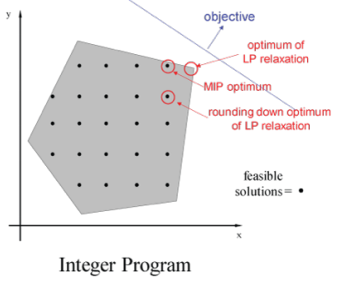
\includegraphics[width=6cm]{integerlinearprogram.png}
\end{tabular}


We can solve this using branch and bounds:

\begin{tabular}{m{12cm}m{6cm}}
    If at the optimal solution of
the linear programming relaxation, one variable is not an integer $x_i =
v$, we create two branches and adding those constraints will only
decrease the upper-bound.
    &
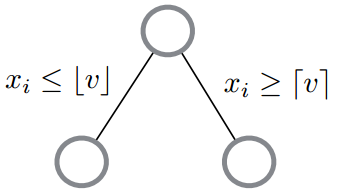
\includegraphics[width=3cm]{branch.png}
\end{tabular}



\subsection{Exam}
\begin{itemize}
    \item Formulate a linear program. 
    \item Be able to transform a LP into standard and slack form. 
    \item Explain and be able to find a initial BFS. 
    \item Apply the simplex algorithm on a small example. (be familiar with the pivoting)
    \item Explain how to detect an unbounded objective.

        $\Rightarrow$ You spot it when you have a var $x_i$ with a
        positive reduced cost in $z$ which always appears in constraints of the form 
        $b_i + x_i = x_n$
\end{itemize}


\section{Lagrangian relaxation}
\subsection{Definition}
The Lagrangian relaxation is a procedure that find a \textbf{lower
bounds}. This
lower bounds will allow to have better performances on the branch and
bounds of the problem starting with an initially good lower-bounds.

\begin{enumerate}
    \item We first relax the problem with the Lagrangian relaxation 
    \item We optimize the $\lambda$ with a sub-gradient algorithm 
    \item We get the optimal $\lambda$ and thus the optimal solution of
        the relaxed problem which is a good lower bounds.
\end{enumerate}

\subsection{Constrained Shortest Path Problem}
In order to represents the concepts discussed in this section, we will
need an example. Lets take the Constrained Shortest Path problem.

\begin{tabular}{m{8cm}m{6cm}}
    \begin{eqnarray*}
        \textrm{minimize } & \sum_{(i,j) \in A} c_{ij} \quad x_{ij} \\
        \textrm{subject to } & \textrm{flow conservation}\\
                            & \sum_{(i,j) \in A } \quad t_{ij} x_{ij} \leq T \\
                             & \forall (i, j) \in A, \quad x_{ij} \in \{0, 1\}
        \end{eqnarray*}

        \begin{itemize}
            \item A example can be to minimize distance with
                \textbf{time constraint} (NP-Hard problem).
        \end{itemize}
& 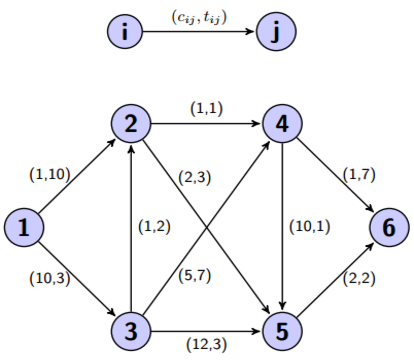
\includegraphics[width=7cm]{lagrangeexample.png}
\end{tabular}


\subsection{Relaxation}

If we remove the resource constraint, the problem is pretty easy. It is
a simple shortest path problem that can be easily resolved with
Dijkstra. What the Lagrangian relaxation does is \textbf{removing the
constraint} and \textbf{adding a new part} in our minimization part.

\begin{eqnarray*}
    L(\lambda) &=& min \sum_{(i,j)\in A} c_{ij} x_{ij} + 
    \textcolor{red}{\lambda \bigg(\sum_{(i,j)\in A} t_{ij} x_{ij} - T
    \bigg)} \\
    %&=& min \sum_{(i,j)\in A} \Big(c_{ij} + \lambda t_{ij}\Big) x_{ij} - \lambda T\\
\end{eqnarray*}

$\Rightarrow$ We now have a simple shortest path problem 
where edges has a weight which is a
mixed value of time and distance for a given value of $\lambda$. 

\begin{itemize}
    \item Using this minimization with different $\lambda$ will return
        different solutions. 

    \item Some of them won't be feasibly and will violate the time
        constraint. If you are lucky one of the solution will be the
        optimal one. (hint: try $\lambda = 2$)
\end{itemize}

\subsection{Lagrangian dual}
Now our objective will be to find the best $\lambda$ in order to have
the best feasible solution (the best we can have with Lagrangian, not
necessarily the best of the actual problem, this algorithm is only used
to have a lower bound). We have our Lagrangian dual: 
$$L* = max_{\lambda} \Bigg( min \sum_{(i,j)\in A} (c_{ij} + x_{ij}) +
\lambda \big(\sum_{(i,j)\in A} (t_{ij} x_{ij}) - T\big) \Bigg)$$

\paragraph{Idea}
The idea, according to Nicolas Houtain, is that 
\begin{itemize} 
    \item we know that as the minimum value are convex and that the max
        value on these minimum value are the point where we pass from 
        unfeasible path to feasible path

    \item So, the max value is the feasible path with minimum value. We
        want to have the first feasible path (it means the minimum
        $\lambda$ with feasible path as minimum value) because it's the
        path where the time constraint have the lower impact on $c_p +
        \lambda (t_P -T)$
\end{itemize}

\subsection{Find best $\lambda$}

\subsubsection{Brute force}
Formulate the minimization problem as a minimization over the set of all 
the feasible path $\rho \in P$:
$$L* = max_{\lambda} \Bigg( min \{ c_{p} + \lambda\big(t_p - T): \rho
    \in P \}\Bigg)$$

\subsubsection{Sub-gradient algorithm}

\begin{enumerate}
    \item Take an initial $\lambda$ and calculate the solution (Dijkstra resolution)
    \item We check if we are on a 
        \begin{itemize}
            \item increasing edge (violation of the constraint) 
            \item or a decreasing edge (constraint is respected). 
        \end{itemize}

        $\Rightarrow$ Depending of that we will respectively move to
        the right or to the left.
\end{enumerate}

\begin{tabular}{m{9cm}m{9cm}}
    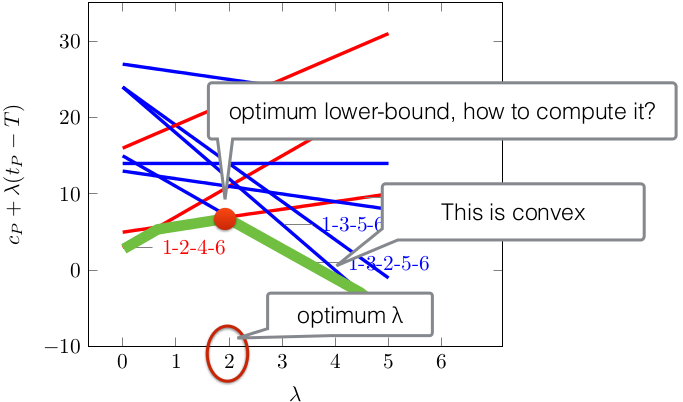
\includegraphics[width=9cm]{lag}
    &
    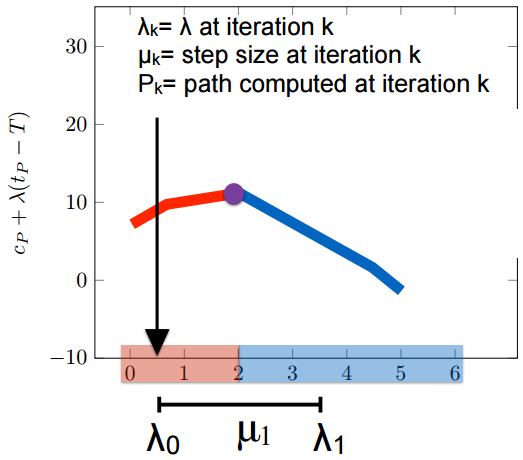
\includegraphics[width=7cm]{lagrangiangraph.png}
\end{tabular}



\paragraph{Computing optimum $\lambda$}
Note that $\lambda_0 = 0$
\begin{enumerate}
    \item At iteration $k$, if $P_k$ violate times constraint increase
        $\lambda$ else decrease it 
        $$\lambda_{k+1} = max(0, \lambda_k + µ_k(t_{P_k} - T))$$

    \item $µ_{k+1} = \frac{1}{k}$
\end{enumerate}

\paragraph{Convergence}

\begin{itemize}
    \item In order for the algorithm to converge we must reduce the size
        of the step at each iteration. 
    \item It is guaranteed to converge if $\mu_{k} \rightarrow 0$ and
        $\sum^{k}_{j=1} \mu_{k} \rightarrow \infty$.
    \item On the other hand the Lagrangian lower bounds has no
        guaranteed to increase at each step.
    \end{itemize}

\paragraph{Pseudo-code}:

\begin{tabular}{m{9cm}m{6cm}}
\begin{lstlisting}[mathescape]
// Result: A lower bound L* and a potentially good (not proven optimal) feasible candidate path P*
L* = $-\infty, \quad k = 0, \quad µ_0=1, \quad \lambda_0 = 0$
P* = shortest path using weights $t_{ij}$
if ($t_{p*} > T$) then
    return 'unfeasible'

while($µ \geq \epsilon$) do
    // Compute shortest path $P_k$ using 
    // weights $c_{ij} + \lambda_k t_{ij}$
    $L_k = c_{P_k} + \lambda_k \bigg(t_{P_k} - T \bigg)$
    if $L_k \geq L*$ then
        $L* = L_k$
        if $P_k$ is feasible then
            $P* = P_k$

    Udate $\lambda_k$ and $µ_k$
    k = k+1
\end{lstlisting}
&
It has not guarantee to find the best
one. But we have a lower-bound at
if P k is feasible then
the end thus we can compute the
« gap »: $$(C_{P_k} - L*)/L*$$
The gap should be non decreasing.
\end{tabular}

\paragraph{Performances}

The Lagrangian relaxation is as good as the linear relaxation. But the
advantage of the Lagrangian one is that it will return feasible solution
during the process.

Typically the lower bounds will evolve along a curve that converge after x steps.

\centerline{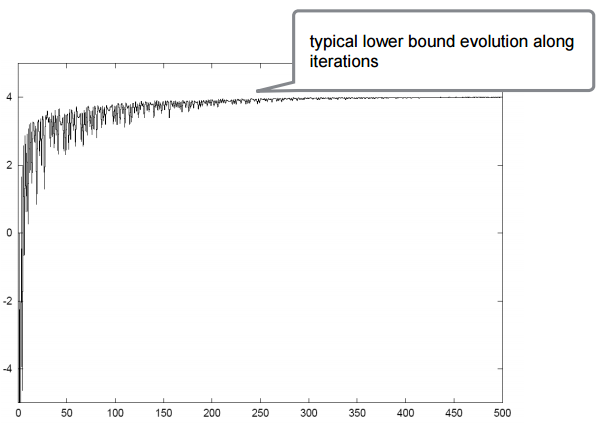
\includegraphics[scale=0.8]{lagrangeconverge.png}}



\section{Network flow}
\subsection{Graph reminder}

\subsubsection{Definitions}

\begin{description}
    \item[A directed graph] is tuple (V, E) where V is the set of vertices 
        and $E \in V x V$ is the set of edges.

    \item[A path] is a suite of distinct nodes $n_0, n_1, ... n_{(k-1)}$ with
        $\big(n_i, n_{(i+1)}\big)$ an
        edge for all $0 \leq i \le k-1$. 

    Node $n_0$ is the origin and node $n_{(k-1)}$ is the
        destination.

    \item[A cycle] is suite of distinct nodes  $n_0, n_1, ... n_{(k-1)}$ with
        $\big(n_i, n_{(i+1)}\% k\big)$ an edge for all $0 \leq i \le k$.
\end{description}

\subsubsection{Graph representation}

\begin{itemize}
    \item Adjacency matrix: The simples one but matrix don't take
        sparsity into account and linear time to iterate over adjacent
        nodes.

    \item Adjacency Lists

        \begin{center}
            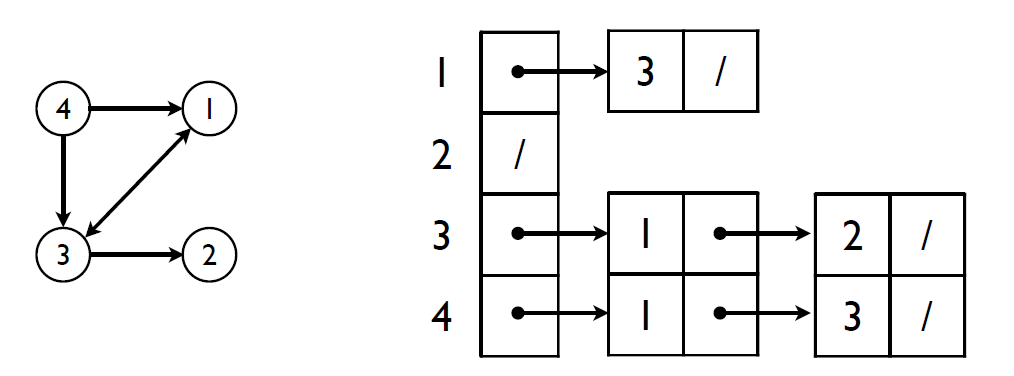
\includegraphics[width=0.3\linewidth]{AdjacencyList.png}
        \end{center}
\end{itemize}


\subsubsection{DFS}

\begin{tabular}{m{7cm}m{5cm}m{3cm}}
    \begin{lstlisting}[mathescape]
DFS(V , E):
    // Initialization;
    Create global variable Color[1..|V |]
    Create global variable Parent[1..|V |]
    for each node $u \in V$ do 
        Color[u] = white
        Parent[u] = Nul
    // Start the search
    for each node $U \in V$ do
        if Color[u] = white then
            Visit(u, V, E)
    \end{lstlisting}
    &
    \begin{lstlisting}[mathescape]
Visit(u, V, E):
    Color[u] = Grey
    for $v \in Adj[u]$ do
        // Explore arc (u, v)
        if Color[v] = white then
            Parent[v] =  u
            Visit(v, V, E)
    Color[u] = black
    \end{lstlisting}
    &
    \begin{itemize}
        \item White: Unvisited
        \item Grey: Not all adjacent edge visited
        \item Black: Fully visited
        \end{itemize}
\end{tabular}

$\Rightarrow$ Say that as we are in a graph, we need to color node that we have
already explored so that we don't reexplore them. 

\paragraph{Complexity}
\begin{itemize}
    \item Init: $O(|V|)$
    \item $O(|V| + |E|)$ : As we have to check every edges at every node
        but we pass on each node once.
\end{itemize}

\subsection{Max flow}

Max flow is a combinatorial problem on Graphs.
He can be solved in polynomial time !

\subsubsection{Definitions}

\begin{itemize}
    \item \textbf{s} is the source and \textbf{t} is the sink
    \item $c(a, b)$ is the \textbf{capacity} between nodes $a$ and $b$.
        ($c(a, b)=0$ if there isn't a edge)

    \item $f(a, b)$ is the \textbf{flow quantity} between node $a$ and
        $b$. (A flow is a vector $f$ such that each composant is associated to a
        pair of nodes.)
$$f(a,b) = -f(a,b)$$ 
\end{itemize}

An \textbf{instance of the Max Flow problem} is characterized by the
graph $G = (V, E)$, the source $s$, the sink $t$ and the vector of
capacity $c$.

\paragraph{Constraints}
\begin{itemize} 
    \item \textbf{Flow conservation} constraint: the
        quantity of water entering into a node (different from
        source and sink) is exactly the same as the quantity of of
        water exiting this node.
        \begin{eqnarray*}
            \forall a\in V\{s,t\} & 
            \sum_{b|(b,a) \in E} \quad f(b,a)  &= \sum_{b|(a,b) \in E}
            \quad f(a,b) 
        \end{eqnarray*}
        Or equivalently
        \begin{eqnarray*}
            \forall a\in V\{s,t\} & 
            \sum_{b \in V} \quad f(a,b)  &= 0
        \end{eqnarray*}

\item \textbf{Capacity} constraint: the flow through each edge does
    not exceed the capacity of this edge.
    \begin{eqnarray*}
        \forall (a,b) \in E & f(a, b) \leq c(a, b)\\
        \forall (a,b) \notin E & f(a, b) \leq 0
    \end{eqnarray*}
\end{itemize}

\paragraph{Flow}
\begin{itemize} 
    \item A \textbf{valid flow} satisfies the two constraints
    \item A \textbf{null} flow is a valid flow where $f(a,b)=0$ for each
        edge
    \item The \textbf{value of a valid flow} is the water quantity out
        of the source. Because of the conservation flow constraint, this
        value is also equal to the quantity entering the sink.
        \begin{eqnarray*}
            v(f) =    \sum_{a \in V |(s,a) \in E} \quad f(s,a)  =
            \sum_{a \in V|(a,t) \in E}
            \quad f(a,t) 
        \end{eqnarray*}

    \item[$\Rightarrow$] The max flow problem is to discover a valid flow of
maximal value
\end{itemize}



\subsubsection{Graphical representation}

\begin{tabular}{m{9cm}m{8cm}}
We usually only represent edges with positive capacity and non
negative flows. We now implicitly add the \textbf{reverse edges} with
capacity 0.
&
    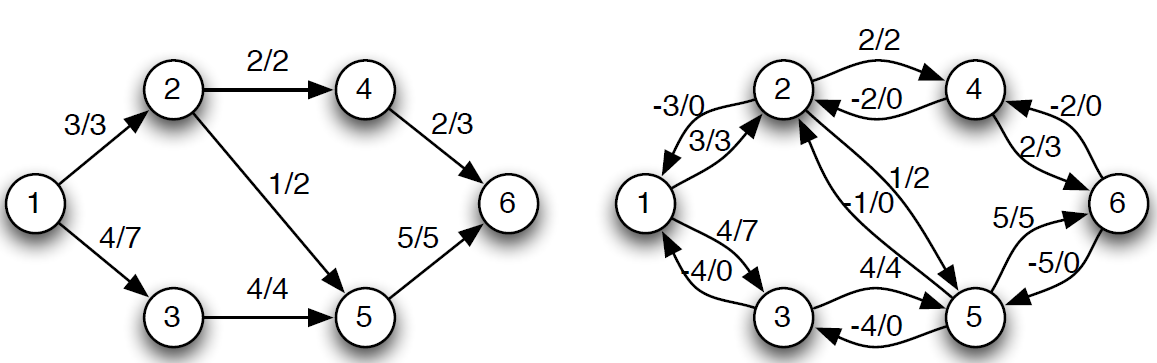
\includegraphics[width=\linewidth]{MaxFlowGraphRepr.png}
\end{tabular}

\begin{tabular}{m{10cm}m{1.5cm}m{1.5cm}}
For bidirectional edges, the reverse edge that we have will have the capacity of the second edge as shown in the example below.
&
    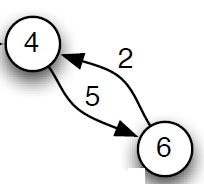
\includegraphics[width=\linewidth]{MaxFlowBidirectionnalRepresentation.png}
    &
    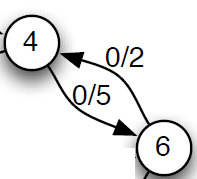
\includegraphics[width=\linewidth]{MaxFlowBidirectionnalRepresentation2.png}
\end{tabular}


\subsubsection{Residual and augmenting path}

\begin{itemize}
    \item \textbf{Residual graph} $G_f = (V, E_f)$ are used to discover paths from the
        source to the sink on which it is possible to push an
        additional quantity of water and so increase the value of the
        flow. 

        \begin{itemize}
            \item This graph is composed of exactly the same nodes as the
                original graph $G = (V, E)$ but the edges may have a different
                direction and a different (residual) capacity.

            \item A edge $(a, b)$ is in the residual only if it is not
                satured (we can add flow):
                $$(a, b) \in E_f \Leftrightarrow f(a, b) < c(a, b)$$

            \item The residual capacity is 
                $$c_f(a, b) = c(a, b) - f(a, b)$$

        \begin{center}
            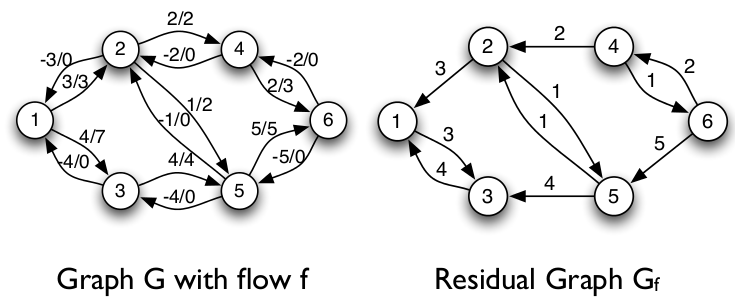
\includegraphics[width=8cm]{residualGraphExample}
            \end{center}

    \item A path joining the source $s$ to the sink $t$ in the residual
        graph $G_f$ is called \textbf{augmenting path}.

        \paragraph{Adding a augmenting path $C$}
            Let $q=c_f(a, b)$, the following
            flow $f'$ is a valid flow with value:
                $$f'(a, b) = \begin{cases}
                    f(a,b) + q & if (a, b) \in C\\
                    f(a,b) - q & if (b, a) \in C\\
                    f(a,b)  & otherwise\\
                \end{cases}$$
        \end{itemize}

\end{itemize}


\subsubsection{Ford-Fulkerson Algorithm}

\begin{lstlisting}[mathescape]
Ford-Fulkerson(V, E, c, s, t):
// Build a vector $f$ with $\frac{|V|}{2}$ entries initialized at 0
    do
        Build the residual graph $G_f$ 
        Find a path $C$ from $s$ to $t$ in $G_f$ 
        if such a path exists then
            Let q be the smallest residual capacity on an edge of path C;
            for every edges $(a, b)$ of path $C$ do
                $f (a, b) = f (a, b) + q$
                $f (b, a) = f (b, a) q$
    while we cannot find a path between $s$ and $t$ in $G_f$ 
    return $f$ ;
\end{lstlisting}

\paragraph{Ford-Fulkerson runtime example}
\begin{center}
    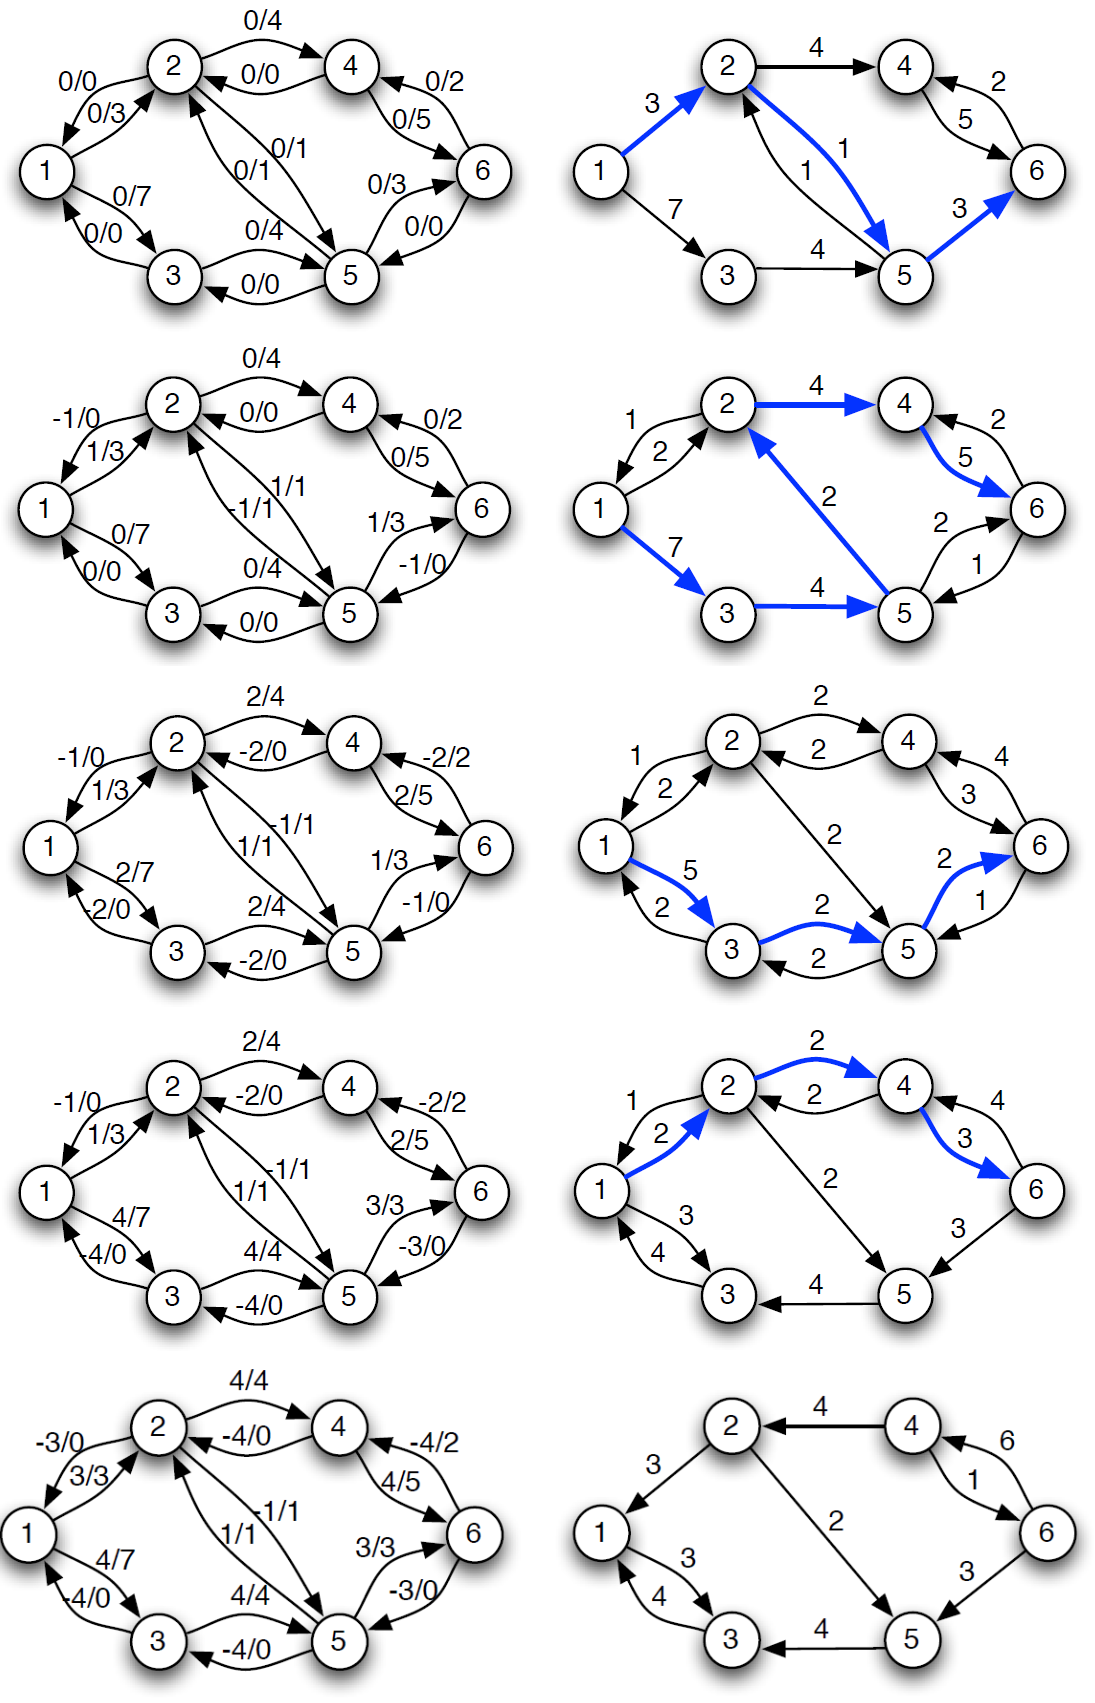
\includegraphics[width=0.55\linewidth]{MaxFlowAlgoExecutionExample.png}
\end{center}

\paragraph{Complexity}
As the complexity of the algorithm is $O(v(f) |E|) = O(|V| |E| U)$ with U the
maximum flow of the graph. 

\begin{itemize}
    \item $O(|V|+|E|)$ to search a augmenting path with DFS. As $|V| - 1
        \leq |E|$, we have $O(|E|)$
    \item Update de residual graph is in $O(|V|)$
    \item In the worst case, we need as many iterations as the value of
        the final maximal flow i.e. $v(f)$

        Note that
        \begin{enumerate}
            \item
                the cut ({s},V-{s}) is, by construction, "intersecting"
                at most $2*(|V|-1)$ edges (one for each vertex that are
                not the source and the direction). Since each edge has
                at most U as value, it gives us that $c(\{s\},V-\{s\}) \in
                O(|V|*U)$.

            \item Since it's a "random" cut, we have that the min cut
                (S,T) have $c(S,T) <= c({s},V-{s})$ (by definition of a
                minimum cut)

            \item From the max-flow/min-cut theorem, you have that value
                of the max-flow v(f) equals the value of the min cut
                c(S,T):

                $$v(f) = c(S,T) \leq c({s},V-{s})$$

                \item Thus, $v(f) \in O(|V|*U), and O(v(f)*|E|) \in
                O(|V|*|E|*U)$.
        \end{enumerate}
\end{itemize}

The complexity is thus not polynomial but
pseudo-polynomial (because the input takes $log(U)$ bits to represent
$U$). 

\subsubsection{Delta-scaling}
In order to be polynomial, we must use
delta scaling where the idea is to augment the flow along a path with sufficiently large
residual capacity ( $\geqslant \Delta$)

\begin{enumerate}
    \item initial $\Delta = 2^{log(U)}$
    \item Let $G_{f,\Delta}$ be $G_f$ with edges with residual capacacity $c_f \geq \Delta$ 

        $\Rightarrow$ Then find augmenting paths in $G_{f,\Delta}$ until not
        possible with current value of $\Delta$. Call this phase a
        $\Delta$-scaling phase.

    \item if $\Delta > 1$ : $\Delta = \frac{\Delta}{2}$ and go to 1.

\end{enumerate}

\begin{lstlisting}
Delta-Scaling :
    delta = X > 1
    while true {
        Filter out all edges with capa < X in residual graph
        if you find an augmenting path :
            delta *= 2
            q = smallest capa of path
            for every edge of path do:
                f(a,b) = f(a,b) + q
                f(b,a) = f(b,a) - q
        else if delta > 1 :
            delta /= 2
        else
            break;
    }
    return result
\end{lstlisting}

\paragraph{Complexity}
$O(|E|^2 log U)$ because 
\begin{itemize} 
        \item $O(|E|)$ augmenting path at each $\Delta$-scaling phase
        \item $O(|E|)$ to discover one augmenting path
        \item $O(Log(U)))$ iteration in scaling.
            
            $\Rightarrow$ As their are a maximum of log(U) iteration with delta scaling, the
            algorithm is of polynomial complexity.
    \end{itemize}

\paragraph{Number of steps in $\Delta$-scaling phase}
\begin{itemize}
    \item Consider \begin{itemize}
                \item the flow $f$ at the end of the $\Delta$-scaling phase
and let v(f) denote its flow value.
                \item $S$ be the set of nodes reachable from $s$ in
                    $G_{f,\Delta}$
                    \end{itemize}
    \item Then $(S,V-S)$ is an s-t cut and by definition of $S$, the residual
capacity of the cut is $c(S,V-S) \geqslant |E|\Delta$

    \item[$\Rightarrow$] If $f*$ is the optimal flow, then $v(f*)-v(f)
        \leq |E|\Delta$.

        \item In the next $\Delta$-scaling phase, each augmentation carries
at least $\Delta$/2 units, so the next $\Delta$-scaling phase can perform at most 2|E|
augmentations
\end{itemize}

\subsection{Min cut}

How much cut do we have to make to partition a graph such that two node
$s$ and $t$, are in different partition. Answer == MaxFlow(s,t)

\subsubsection{Definitions}

\begin{itemize}
    \item A cut is bipartition of a set V formed of two disjoint sets
        $S$ and $T$ such that $V$ is the union of $S$ and $T$.
        $$S \cup T = V \quad \quad S \cap T = \emptyset $$

    \item A cut in a network is a bipartition ($S, T$) of the nodes such
        that the source is in the set $S$ and the sink is in the set $T$
        $$S \cup T = V , s\in S\quad \quad S \cap T = \emptyset, t \in
        T$$

    \item The capacity of a cut (S, T) is the capacity of the edges
        linking
        a node from S to a node in T.
        $$c(S, T) = \sum_{a\in S} \sum_{b \in T} c(a, b)$$

    \item The net flow of a cut ($S, T$) is the quantity of flow
        (positive or
        negative) from a node in S to a node in T.
        $$f(S, T) = \sum_{a\in S, b\in T} f(a, b)$$

\end{itemize}

\paragraph{Example}

        \begin{tabular}{m{5cm}m{6cm}}
            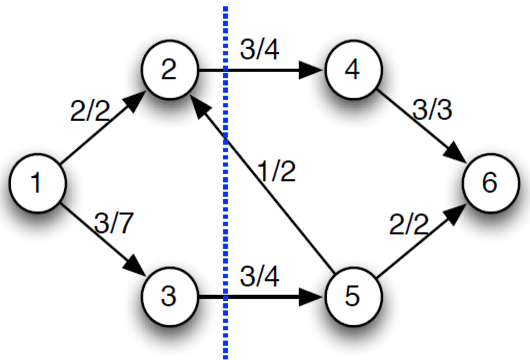
\includegraphics[width=\linewidth]{CutDefinition1.png}
            &
                \begin{eqnarray*}
                    c(\{1, 2, 3\}, \{4, 5, 6\}) & =& 8\\
                        \\
                        f(\{1,2, 3\}, \{4, 5, 6\}) & =& f(2, 4) +
                        f(2, 5) + f(3, 5)\\
                        & =& 3 - 1 + 3 \\
                        & =& 5
                    \end{eqnarray*}
        \end{tabular}


\subsubsection{Net flow of cut with value of flow}
\begin{center}
    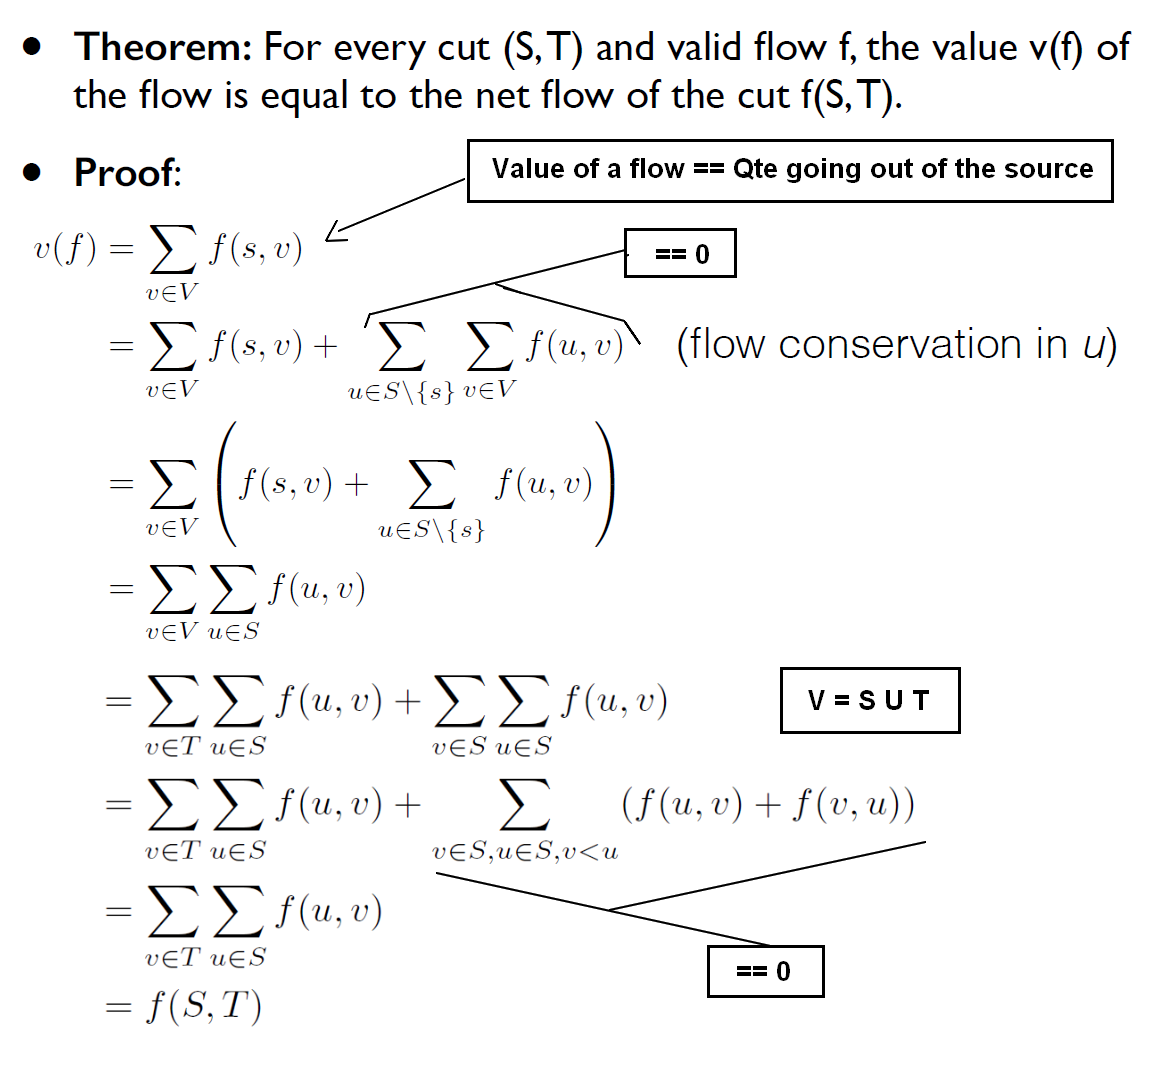
\includegraphics[width=0.7\linewidth]{CutProof.png}
\end{center}

\subsection{Max flow - min cut theorem}
Given a feasible flow $f$, these properties are equivalent:
\begin{enumerate}
    \item $f$ is maximum flow in $G$
    \item The residual graph $G_f$ has no augmenting path
    \item There exists a cut ($S, T$) with capacity $c(S, T) = v(f)$

        \textit{It means that there is a cut which only take edge with
        the bottleneck}
\end{enumerate}

\begin{itemize}
    \item[$1\Rightarrow2$] If this path would exists, we could build a
        larger flow (contradicts the fact that it is maximal).

    \item[$2\Rightarrow3$] Let $u \in S$ and $v\in T$:
        \begin{itemize}
            \item if $(u, v) \in E$ is an edge then $f(u, v) = c(u, v)$
                otherwise $s$ could reach $v$ in $G_f$ 
            \item If $(v, u) \in E$ is an edge then $f(u, v) = 0$
                otherwise $s$ could reach $v$ in $G_f$ .
            \item Otherwise, $f(u, v) = 0$ since no flow can flow between
                two nodes not linked by an edge
        \end{itemize}
        \begin{center}
    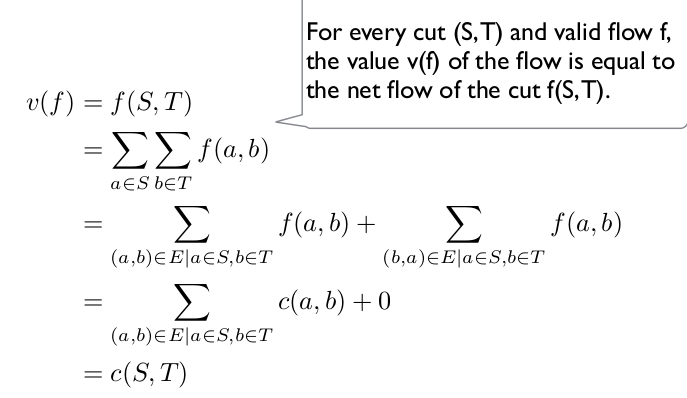
\includegraphics[width=11cm]{23.png}
    \end{center}

    \item[$3\Rightarrow1$] The value of flow cannot exceed the capacity of one of its
        cut.
        \begin{center}
    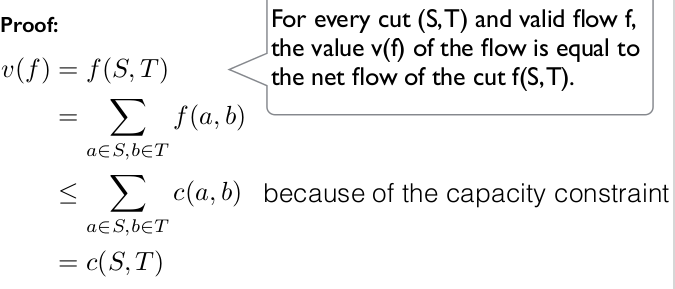
\includegraphics[width=10cm]{31.png}
    \end{center}
    \end{itemize}

$\Rightarrow$ A flow with a value equal to the capacity of one of its cut is thus
maximum.

\subsubsection{Proof that the cut is minimal}
For any feasible flow $f$ of value $v(f)$, there exists a cut $(S,T)$ such
that the flow $f(S,T)$ that crosses the cut is equal to $v(f)$. Since for
any feasible flow we have $f(S,T) \leqslant c(S,T)$, if you find a flow $v(f) =
f(S,T) = c(S,T)$, then you can't find a cut with capacity less than
$c(S,T)$ (the flow $v(f)$ would still have to pass through the cut because
it's a valid flow). Hence any cut with $v(f) = c(S,T)$ is minimal.

\subsection{Min cost flow}
\begin{enumerate}
    \item Start with a flow of zero
    \item  Find an s-t path in G f with minimum weight
    \item  Augment along this path as much as possible (limited by
        smallest
        residual capacity of the path).
    \item  Repeat two previous steps until initial demand B of the source
        is met.
\end{enumerate}

\begin{figure}[!ht]
    \centering
    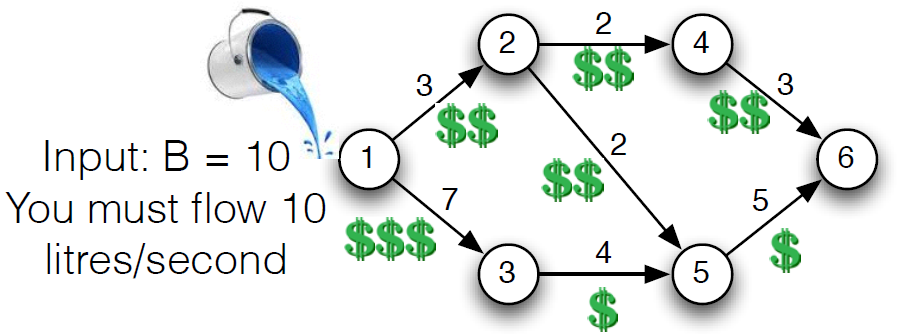
\includegraphics[width=0.5\linewidth]{minFlow.png}
\end{figure}

Be careful that in some problem negative weight may be used and infinite
loop must thus be avoided. => Use the Moore-Bellman-Ford algorithm
\url{https://en.wikipedia.org/wiki/Bellman%E2%80%93Ford_algorithm} 



\subsection{Scheduling}

\begin{tabular}{m{8cm}m{7cm}}
4 persons must give a seminar in a
single room with their possible slots.
\begin{itemize}
    \item  Alice (11h, 13h); Benoit (9h, 10h, 13h);
        Clotilde (9h, 11h, 13h) and Dany (11h, 13h).
\end{itemize}
&
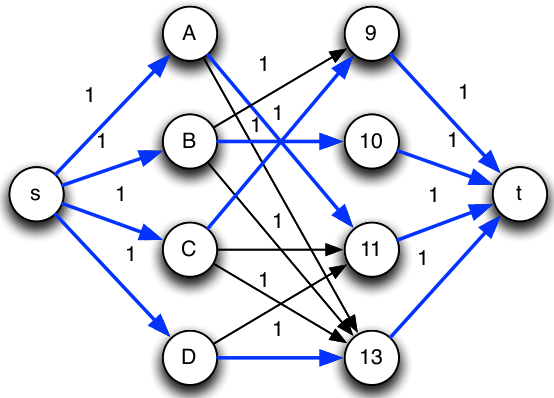
\includegraphics[width=6cm]{flowSchedul.png}
\end{tabular}


\subsection{Flows and Linear programming}
A flow can be describe as a LP since:
\begin{itemize}
    \item Maximize the outgoing flow from source
    \item Under two constraint : capacity and flow conservation
\end{itemize}


\section{Greedy and approximation algorithms}

\subsection{An activity-selection problem}
\begin{tabular}{m{6cm}m{10cm}}
    Find the max number of activities that do not
    overlap in time : 
    $$\forall i,j \quad selected: \quad s_i \geq f_j  \quad or \quad s_j \geq f_i$$
    &
\begin{itemize}
    \item $s_i$ = start time of activity
    \item $f_i$ = end time activity (not that activities are 
        sorted such that $f_i \leq f_{i+1}$)
\end{itemize}
\end{tabular}

\begin{enumerate}
    \item \textbf{Reduction} to the maximum independent set problem where 
        we find the maximum set of vertices in a graph such that
        to vertices selected are not adjacent.

        \begin{tabular}{m{10cm}m{3cm}}
            \begin{itemize}
                \item The reduction is done by add an edge between $i$ and $j$ if
                    activities overlap in time: 
                    $$s_i < f_j \quad and \quad s_j < f_i$$ 
            \end{itemize}
            Note that the maximum independent set problem is NP-Hard problem
            &
            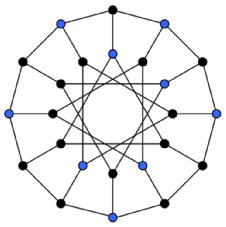
\includegraphics[width=3cm]{img/independant}
        \end{tabular}


    \item \textbf{Dynamic programming}: select a maximum size subset of mutually
        compatible activities from $S_{ij}$, for $0 \leq i < j \leq n+1$,
        knowing that all other $S_{ij}$ are empty.
        \[
            c[i, j] = 
            \begin{cases} 
                0 & \text{if } S_{ij} = \emptyset \\
                max_{\substack{i<k<j \\ a_k \in S_{ij}}} \{c[i, k] + c[k, j] + 1\}  & \text{if } S_{ij} \neq \emptyset
            \end{cases}
        \]
        \begin{itemize}
                %TODO
            \item Time complexity: 
            \item Space complexity: 
        \end{itemize}

        \paragraph{Improvement to a greedy}
        $$a_m\textrm{ such that }f_m = min\{f_k: a_k \in S_{ij}\}$$
        \begin{itemize}
            \item Obs.1: $a_m$ is used in some maximum-size subset of
                mutually compatible activities of $S_ij$

                Proof (Sketch):
                \begin{small}
                    Suppose $A_{ij}$ an optimal set of $S_{ij}$ . Take
                    the first activity of $A_{ij}$ (assume it is $a_k$ with $k \neq m$). We
                    can safely replace $a_k$ with $a_m$ because $f_m \leq f_k$.
                \end{small}

            \item Obs.2: The subproblem $S_{im}$ is empty, so that choosing
                $a_m$ (in the recurrence) leaves the subproblem $S_{mj}$ as the
                only one that may be nonempty.
        \end{itemize}

        %TODO new recurrence equation

    \item \textbf{Greedy algorithm}
        \begin{lstlisting}[mathescape]
n $=$ nbrActivities
A $= a_1$
i $= 1$

for m $\leftarrow$ 2 to n do
    if $s_m \geq f_i$ then
        A = $A \cup a_m$
        i =$m$

return A
        \end{lstlisting}
\end{enumerate}


\subsection{Greedy}
At each decision point, the algorithm makes
a \textbf{local optimum choice} in the hope that it is a global
optimum choice.
\begin{itemize}
    \item For some problem it's the case
    \item For other it's not and sometimes we can 
        have a guarantee how
        \textit{suboptimal} we can be.
\end{itemize}


\subsection{Minimum Spanning Tree (MST)}

\subsubsection{Definition}
\begin{itemize}
    \item A \textbf{cut} (S,V-S) of an undirected graph
    \item An edge (u,v) \textbf{cross} the cut (S,V-S) if one of its
        endpoints is in S and the other in V-S
    \item A cut \textbf{respects} a set A of edges if no edge in A crosses
        the cut.
    \item An edge is a \textbf{light edge} crossing a cut if its weight is
        the minimum of any edge crossing the cut. (can be
        more than one in case of ties).
\end{itemize}

\subsubsection{Theorem}
\begin{itemize}
    \item[LET]
    \item $G=(V,E)$ a undirected graph with weight function $w$ on $E$.
    \item $A \subseteq E$ included in some MST for $G$.
    \item $(S, V-S)$ be any cut of $G$ that respect $A$
    \item $(u,v)$ be a light edge crossing $(S, V-S)$
    \item[THEN]
    \item edge $(u, v)$ is safe for $A$
\end{itemize}

\paragraph{Proof}
Let $T$ be a minimum spanning tree that includes $A$, and assume
that $T$ does not contain the light edge $(u,v)$, since if it does we
are done.

\begin{enumerate}
    \item Because $(u,v)$ are on opposite sides
        of the cut $(S,V-T)$ that respects $A$,
        there is necessarily some edge $(x,y)$
        on path $p$ also on opposite sides of
        the cut.

    \item We can form an other MST $T'$ by
        removing $(x,y)$ and adding $(u,v)$ from
        $T$. Because when considering $A$,
        $(u,v)$ is a light edge, $(x,y)$ cannot be
        cheaper than $(u,v)$ (by definition of a
        light edge).
\end{enumerate}


\subsubsection{Algorithm}

\begin{lstlisting}[mathescape, caption=Generic-MST(V\,E\,c\,s\,t)]
A = $\emptyset$
while A does not form a spanning tree do
    find an edge $(u, v)$ that is safe for A
    A = A $\cup \{(u, v)\}$

return A
\end{lstlisting}

\begin{itemize}
    \item \textbf{Kruskal}  
        
        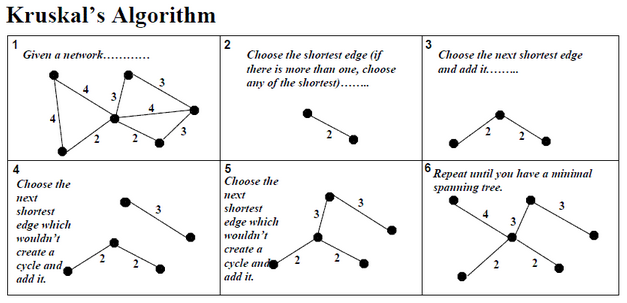
\includegraphics[width=14cm]{img/kruskalAlgo}
    \item \textbf{Prim} 
        
        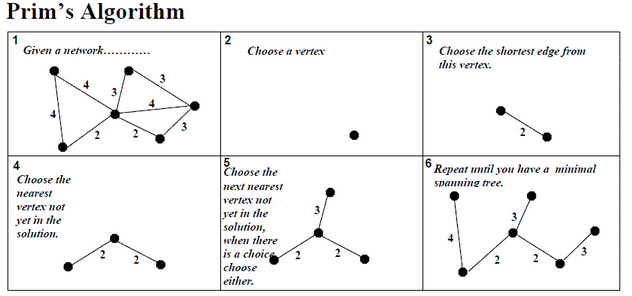
\includegraphics[width=14cm]{img/primAlgo}
\end{itemize}

\subsubsection{Implementation using disjoint-set forests}
Kruskal and prim can be implemented in $O(E \times log(V))$

\begin{lstlisting}[mathescape, caption=MST-Kruskal(G\,w)]
A = $\emptyset$
for each vertex $v \in V$ do
    Make-Set-(v)

sort the edge of $E$ into non decreasing order by weight $w$
for each edge $(u,v) \in E$ taken in non decreasing order by weight do
    if Find-Set(u) $\neq$ Find-Set(v) then
        A = A $\cup \{(u, v)\}$
        Union(u,v)

return A
\end{lstlisting}

\begin{center}
\begin{tabular}{m{7cm}m{7cm}}
    \begin{lstlisting}[mathescape]
MAKE-SET(x)
    X.p = x
    x.rank = 0

FIND-SET(x)
    if x $\neq$ x.p
        x.p = fIND-SET(x.p)
    return x.p
    \end{lstlisting}
    &
    \begin{lstlisting}[mathescape]
UNION(x, y)
    LINK(FIND-SET(x), FIND-SET(y))

LINK(x, y)
    if x.rank > y.rank
        y.p = x
    else 
        x.p = y
        if x.rank == y.rank
            y.rank = y.rank + 1
    \end{lstlisting}\\
    $\rightarrow$ Path compression
    & 
    $\rightarrow$ Union by rank
\end{tabular}
\end{center}

\begin{itemize}
    \item \texttt{Sort} in $O(E \times log(E)) = O(E \times log(V^2)) = O(E \times log(V))$
    \item \texttt{Make-Set(x)}: make a set with $x$
    \item \texttt{Find-Set(x)}: return pointer to the set containing $x$

        \paragraph{O(1)} is assured by using \textbf{path compression}.

        \begin{tabular}{m{11cm}m{3cm}}
            During Find-Set operation, make each node
            on the find path point directly to the root
            &
            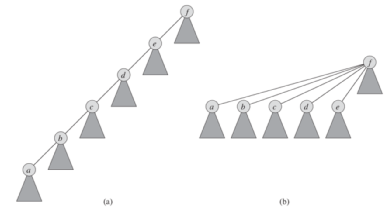
\includegraphics[width=3cm]{img/compression}
    \end{tabular}


    \item \texttt{Union(x, y)}: merge two sets (can't have a duplicate element
        because of set)

        \paragraph{O(1)} is assured by using \textbf{union by rank}.

        \begin{tabular}{m{11cm}m{3cm}}
            Make the root of the tree with the fewer nodes points to
            the root of the tree with more nodes.
            &
            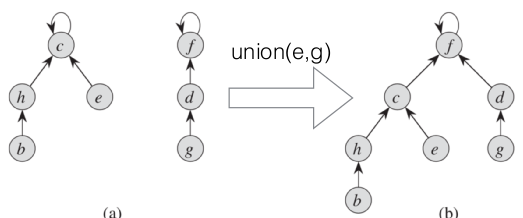
\includegraphics[width=4cm]{img/union}
    \end{tabular}
\end{itemize}

\begin{itemize}
    \item The time complexity of $m$ (> n) operations on $n$ objects
        using Disjoint-set forests implemented with path
        compression and union by rank $i$: 
        $$\Theta(m \quad \alpha(m,n))$$
    \item $\rightarrow \alpha(m, n)$ is the inverse Ackermann's function. 
        In fact, it's less than 5 for any practical input size $n$
\end{itemize}

\subsection{Approximation}

\subsubsection{Approximation ratio}
An algorithm for a problem has an \textbf{approximation ratio} of $\rho(n)$ if
for any input size $n$, the cost $C$ of the solution is within a factor
$\rho(n)$ of the cost C* of an optimal solution.
$$max(\frac{C}{C*}, \frac{C*}{C}) \leq \rho(n)$$

\paragraph{Set cover example}
Minimum set of vertices such that each
edge of the graph is incident to at least one vertex of
the set.

\begin{lstlisting}[mathescape, caption=Greddy set cover]
C = $\emptyset$
E' = G.E
while E' $\neq \emptyset$ do
    $(u, v)$ be arbitrary edge of E'
    C = C $\cup \{u, v\}$
    remove from E' every edge incident on either $u$ or $v$

return C
\end{lstlisting}

\begin{itemize}
        \item Let $A$ the set of edges selected arbitrary. Vertices in
            $A$ are not adjacent (by construction). Thus to cover those
            vertices we need at least 
            $$|C*| \geq |A| \quad \textrm{vertices in an optimal
            cover}$$

        \item[$\Rightarrow$] $|C| = 2 |A| \quad \Leftrightarrow |C| \leq
            2 |C*|$, so            $\rho(n) = 2$
\end{itemize}


\subsubsection{Approximation scheme}
An approximation Scheme is an optimization algorithm also taking as input a value 
$\epsilon > 0$ such that for any fixed $\epsilon$ the scheme is a
(1+$\epsilon$)-approximation algorithm.

\begin{itemize}
    \item A polynomial-time approximation scheme: for any fixed
        $\epsilon > 0$, run time is polynomial in the size $n$ of its input
        (e.g. $O(n^{2/\epsilon} )$)
\begin{center}
    $\Rightarrow$ if $\epsilon$ decreases by a constant factor (say divided by 2),
the running time increases by more than a constant
factor!
\end{center}

    \item A fully polynomial-time approximation scheme:
        polynomial run time both in $1/\epsilon$ and in it’s input size
        (e.g. $O((1/\epsilon)^2 n^3)$ )
\begin{center}
    $\Rightarrow$ if $\epsilon$ decreases by a constant factor (say divided by 2),
    the running time increases by a constant factor (4)!
\end{center}

\end{itemize}

\paragraph{Subset-sum example}
\begin{itemize}
\item $S= \{x_1,...,x_n\}$ a set of positive integers and $t$ a positive integer 
    \item We want to
maximize $\sum x \in S$ subject to $\sum x \in S \leq t$
\end{itemize}


The idea trim each list after is has been created. If two
values are closed enough, since we want an
approximation don’t keep both of them. Let $\delta$ be the
trimming parameter with $0 < \delta < 1$.

\begin{tabular}{m{7cm}m{7cm}}
\begin{lstlisting}[mathescape]
TRIM(L, $\delta$):
    res = \{$y_1$\}
    last = $y_1$
    for i in 2 to m :
        if $y_i > last * (1+\delta)$  // Because L is sorted
            res.append($y_i$)
            last = $y_i$
    \end{lstlisting}
    & 
    \begin{itemize}
        \item $10, 11, 12, 15, 20, 21, 22, 23, 24, 29$
        \item become for $\delta = 0.1$ : $10, 12, 15, 20, 23, 29$
    \end{itemize}
\end{tabular}

For every element $y$ removed, there is an element $z$ that approximates
it: $$\frac{y}{1+\delta} \leq z \leq y$$




\subsection{Exam}
\begin{itemize}
    \item All theoretical notions introduced (proofs, etc).
    \item Design a greedy algorithm
    \item MST: I give you a new MST greedy algorithm. You
        should be able argument whether it is correct or not.
    \item Design a simple approximation scheme, compute it’s
        approximation ratio
    \item I give you a complexity of an approximation scheme.
        You should be able to tel me if it is fully polynomial.
\end{itemize}


\section{Local search}

\subsection{Generic Local Search}
\begin{tabular}{m{9cm}m{7cm}}
\begin{enumerate}
    \item An initial solution s
    \item N(s) is the neighborhood of s
    \item L(N(s), s) is the set of legal moves from a solution s
    \item S() selects the move in the legal moves
\end{enumerate}
&
\begin{lstlisting}[mathescape]
Procedure LocalSearch(f,N,L,S,s):
    s* = s
    for k = 1 to MaxTrials do
        if sastifiable(s) $\wedge$ f(s) < f(s*) then
            s* = s
        s = S(L(N (s), s), s)
    return s*
\end{lstlisting}
\end{tabular}

\subsection{Improvement Heuristic}
We can improve this algorithm with two heuristics:
\begin{itemize}
    \item  \textbf{L-Improvement} will only accept moves that improve the solution
    \item \textbf{S-Best} will select one on the move randomely in case of tie.
\end{itemize}

\subsection{Local Minima}

A big problem with local search is that you can be stuck in a local minima(maxima) for a minimization problem(maximimzation).
We have two solutions to get ou of the local minima(maxima) for that:

\begin{tabular}{m{10cm}m{3cm}}
\begin{itemize}
    \item We can accept to \textbf{degrade the solution}.
    \item \textbf{Enlarge the neighborhood}.
\end{itemize}
&
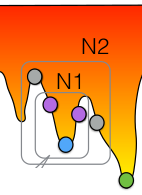
\includegraphics[width=2cm]{localMax}
\end{tabular}

\subsubsection{Degrade the solution}

\paragraph{Constraints types}
\begin{itemize}
    \item \textbf{Hard Constraints} much be respected at all
        time during the local search. (They are enforced at
        initialization)

    \item \textbf{Soft Contstraints} are the constraints that
        can be violated during the search in order to find
        better solutions.
\end{itemize}

For the sudoku example we execute swaps between cases to try to
lower the number of soft constraints violated. Adding more
constraints in the hard constrains makes the initialization
harder but makes the local search process easier.

\paragraph{Tabu meta heuristic}

\begin{itemize}
    \item Whenever you perform a move, this move becomes tabu for a certain
        duration(number of iteration). 
    \item So, when you are stuck in a local minima the
        algorithm keeps iterating between a couple of moves without finding a
        better solution. By making a move tabu you force it to chose some other
        point and escape from the  local minima.

    \item[$\Rightarrow$] If your neightboord is connected and you let the tabu search run
        indefinatly with a long enought tabu periode your algorithm will end up
        finding the optimal solution
\end{itemize}

\paragraph{Improvement on tabu search}
\begin{enumerate}
    \item \textbf{Aspiration}: A move is not considered tabu if it can lead to
        the best so far objective violation.
        So, you not only consider the non tabu moves but you also consider the best
        tabu moves if it improve your best solution and get out of a
        minima.
        
    \item \textbf{Restart}:
        Every X iteration you change randomly some variables in you current
        solution and you restart the from that point. This allows you to travel
        further in the search space in order to maybe find a better solution far
        from the position you were before.
\end{enumerate}


\subsubsection{Enlarge the neighborhood}

\paragraph{Connected Neighborhood}
A neighborhood is connected if and only if for each
solution $s$, there exists a path to an optimal solution $s*$.


This means that if you make the right moves, your neighboord is large
enought to find the optimal solution. However having a connected
neighboord doens't means you will find the optimal solution(in case you
don't make the right moves because of a bad heuristic for
instance).

\begin{itemize}
    \item You don’t necessarily need a restarting strategy (even thought
        this can improve the time to find the best solution)
    \item Randomized heuristics where there is a non zero
        probability of accepting a neighbor$ k \in N(s)$ for each
        solution $s$, may be guaranteed to reach an global
        optimum (example: simulated annealing).
\end{itemize}

\subsection{TSP move}
In order to improve a tour, we can use:

\begin{tabular}{m{3.5cm}m{11cm}}
    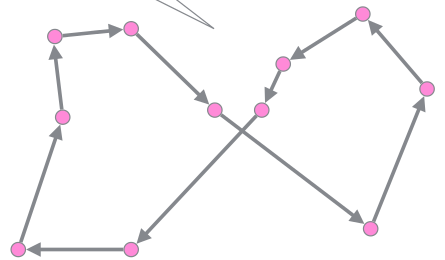
\includegraphics[width=4cm]{tsp}
    &
\begin{itemize}
    \item 2-opt which is an algorithm that swap two edges
        to find a better solution.
        \begin{center}
    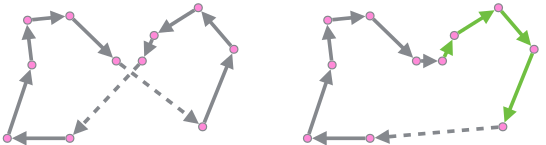
\includegraphics[width=8cm]{2-opt}
        \end{center}
    \item 3-opt
    \item ...
    \end{itemize}
\end{tabular}
    Note that in practice, the 4-opt is too big to 
    compute.

\subsubsection{Sequential k-opt}

As k-opt is computationally too intensive, we
use \textbf{sequential k-opt}.

\begin{itemize}
    \item A k-Opt move is called sequential if it can be described
        by a path alternating between deleted and added
        edges.
        \begin{center}
    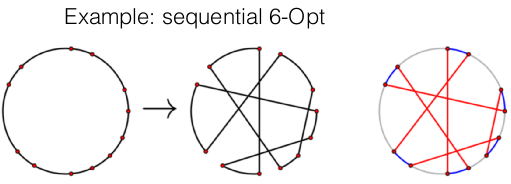
\includegraphics[width=8cm]{6-opt}
        \end{center}

\end{itemize}

The idea is to build greedily a k-Opt move (maybe not the best
move in the k-opt neighboor). At each
step we compute the « gain » of applying it. i.e. the (k
+1)-sequential move is an extension of the k-
sequential move,...

\begin{tabular}{m{10cm}m{6cm}}
$\Rightarrow$ We will start this algorithm with different k's and use the one that gives use to most gain.
&
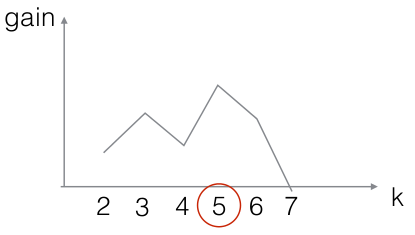
\includegraphics[width=5cm]{linkernighan}
\end{tabular}

\subsubsection{Lin-Kernighan algorithm}
\begin{enumerate}
    \item Let T be the current tour. At each iteration step the
        algorithm attempts to find two sets of edges

        \begin{enumerate}
            \item  We build a set X and Y of edges such that X are the
                deleted edges and Y are the added edges. The edges of X
                are called out-edges and edges of Y are called
                in-edges.

                $\Rightarrow$ If the edges of X are deleted from T and replaced by the
                edges of Y , the result is a better tour.                 
            \item Those edges are
                added elements by elements(empty at start).

        \end{enumerate}
\end{enumerate}

\paragraph{Criteria}

We could start the algorithm just like that but we don't want it to run
forever. This is why we add some \textbf{criteria} to make is sufficiently
efficient.

\begin{itemize}
    %TODO criteria!
    \item \textbf{Sequential exchange criterion}: 
        The sequence $(x1, y1, x2, y2,..., xk, yk)$
        constitutes a chain of adjoining edges.
        $$x_i = (t2i -1, t2i), \quad y_i = (t2i, t2i+1), \quad x_{i+1} =
        (t2i+1, t2i+2)$$

        There must be an added edge followed by a deleted edge.

        \begin{itemize}
            \item[$\Rightarrow$] It's a necessary (but not sufficient) condition that the
        exchange of edges X with edges Y results in a tour is that the
        chain is closed.
    \end{itemize}

    \begin{center}
        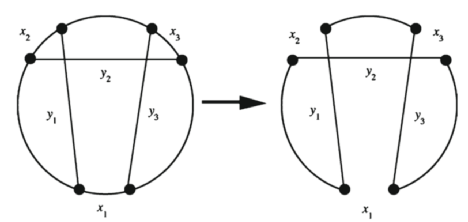
\includegraphics[width=8cm]{seqCriteria}
        \end{center}

\item \textbf{Feasibility criterion}: 
        The resulting configuration must be a cycle.

    \begin{center}
        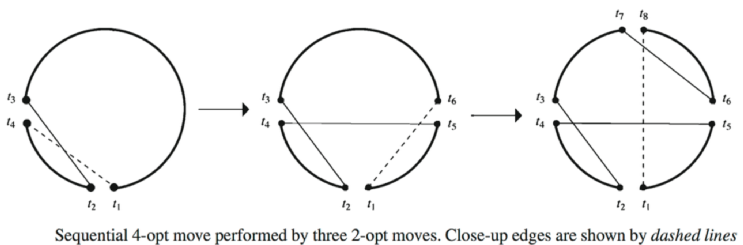
\includegraphics[width=13cm]{feasibleCriteria}
        \end{center}

    \item \textbf{Positive gain criterion}:
        We chose the set Y of edge so that we gain from the nex
        configuration(If the changes gives us a worst solution than the
        one we had before it is not interresting)

    \item \textbf{Disjunctivity criterion}:
        X and Y disjoint(You can't add a deleted edge or you can't
        delete an added edge).

    \item \textbf{Candidate set criterion}:
        When looking for a new edge in Y we limit ourself to only
        considere the 5 nearest neighbors of the vertice.

\end{itemize}

\subsubsection{ATSP reduction to TSP}
Asymetric traveler salesman problem (ATSP)
means that the weight of the edge from A to B isn't necceseraly the
same as the one from B to A. To reduce this problem to the simple TSP we
double every every vertice and put an -inf weight to it.

\begin{center}
    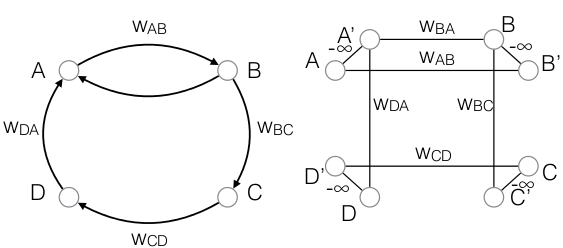
\includegraphics[width=9cm]{ATSP}
\end{center}


\subsection{Vehicle Routing Problem}

\begin{tabular}{m{9cm}m{7cm}}
    This a local search problem mixing the bin packing problem and the TSP problem.
    &
    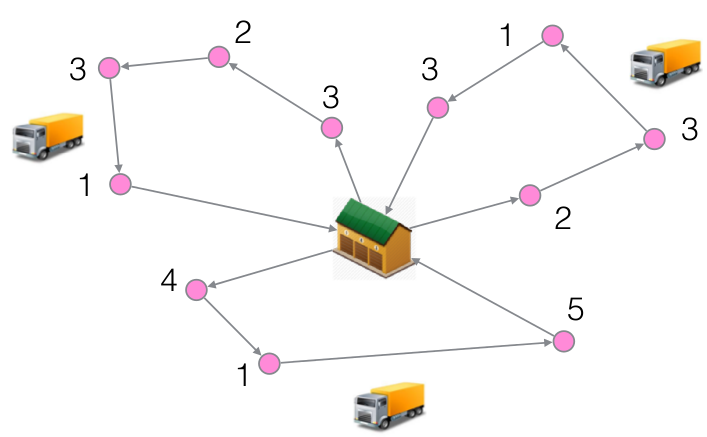
\includegraphics[width=5cm]{vehicle}
\end{tabular}

We have two types of initializations for this local search:
\begin{itemize}
    \item \textbf{Saving Heuristics}

        \begin{tabular}{m{6cm}m{6cm}}
            \begin{enumerate}
                \item We start with a vehicles \textbf{for each}
                    customer.

                \item Iteratively merge routes to
                    decrease the total distance without exceeding the
                    capacity until no more routes can be
                    merge without violating the capacity constraints.
            \end{enumerate}
            & 
            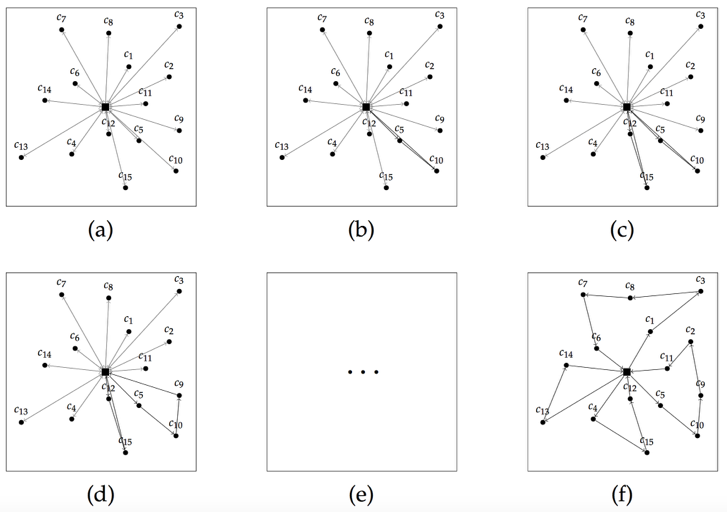
\includegraphics[width=8cm]{saving}
        \end{tabular}

    \item \textbf{Sweep Heuristic} 

        \begin{tabular}{m{6cm}m{6cm}}
            \begin{enumerate}
                \item  Start with a ray centered at the depot. Turn the
                    ray around the depot and every time we cross a
                    customer with the ray we add it to the current
                    cluster.
                \item If the nest customer exceed the capacity we start a new
                    cluster.
            \end{enumerate}
            & 
            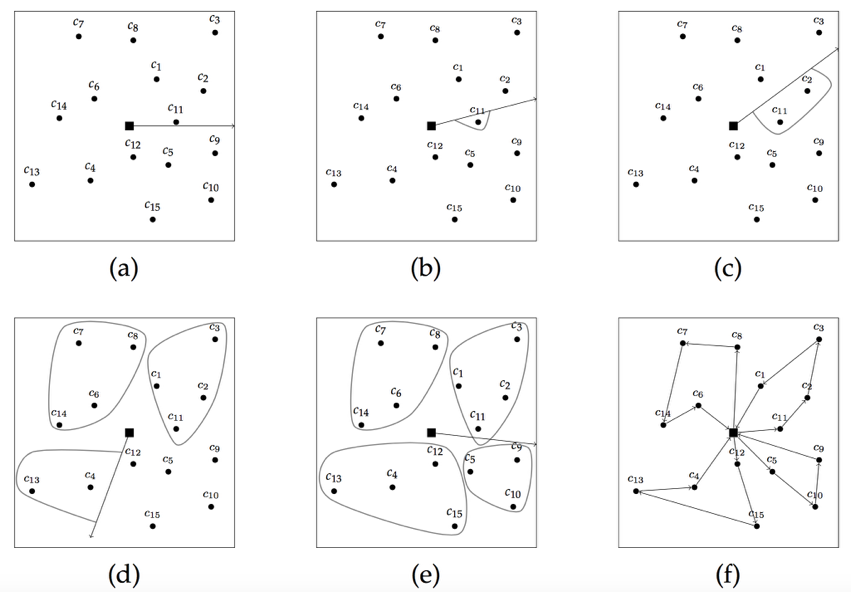
\includegraphics[width=8cm]{sweep}
        \end{tabular}
\end{itemize}

\subsection{Scheduling moves}

\begin{itemize}
    \item Given a set of activities that can not be interrupted and
        that have a certain length and a certain resource need.
    \item A resource with capacity $C$
    \item[$\Rightarrow$] How to minimize the total duration withtou
        exceeding the total capacity.
\end{itemize}

\subsubsection{Iflat-IRelax algorithm (LS)}

We iterativelay flatten then Relax.
\begin{enumerate}
    \item \textbf{Flatten} : We add strong precedences constraints until
        the capacity constrains is satisfied.

        Note that we assume that each
        activity starts as soon as possible while satisfying
        the precedence constraints.

    \item \textbf{Relax} : We remove some precedences randomly on the critical
        path.

        The critical path is that path that is the longest in the
        schedule(the one that makes the schedule the longer).
\end{enumerate}

\subsection{Eternity II}
\begin{itemize}
    \item 16x16 edge matching puzzle
    \end{itemize}

\subsubsection{Swap and rotate}

\begin{enumerate}
    \item Remove $m$ pieces from non edge adjacent positions(up to $n^2/2$ ) 
    \item Replace them optimally:

        \begin{enumerate}
            \item Check score to place them each optimally in holes (by
                check the number of correct adjacent edges)
            \item This generate a complete weighted bipartite graph
                between the removed pieces and holes that we can solve
                thanks to a maximum assignment problem.

                $\Rightarrow$ The size of the Neighborhood is
                exponential but it can be optimally explored in
                polynomial time. (Hungarian algorithm $O(m^3)$)
                \end{enumerate}
\end{enumerate}


\subsection{OscarR CBLS}
\textbf{OscarR CBLS} is a library for local search.
\begin{itemize}
    \item You add the constraints and the objective function and it will
        compute the violations and the delta's for you.
    \item With this you can focus more on the search process(moves and meta-heuristics).
\end{itemize}

\subsection{Exam}
\begin{itemize}
    \item Be able to explain the principle of local search
    \item Be able to implement a simple search with swap-
        moves and a tabu-search meta-heuristic
    \item Be able to suggest a neighborhood for a new problem
        and discuss/prove it it is connected or not.
    \item Be able to explain and apply moves for:
        \begin{itemize}
            \item TSP (Lin-Kernighan) and vehicle routing,
            \item scheduling,
            \item eternity
        \end{itemize}
\end{itemize}


\section{Constraint programming}

\subsection{CP Advantage}
\begin{itemize}
    \item Rich modeling language:
        \begin{itemize}
            \item  integer variables, set variables, graph variables
            \item  library of constraints (not necessarily linear)
        \end{itemize}
    \item  Fast prototyping
    \item  Easy to adapt/change a model
    \item  Extensible (you can create new constraints)
    \item  Great framework to hybridize with other techniques
\end{itemize}

\subsection{Description}

\begin{itemize}
    \item \textsc{Model} : Describe real world problem with
        \begin{itemize}
            \item \textbf{Variables} : $X = \{x_1, x_2,\cdots, x_n\}$

            \item \textbf{Domains} : $D = \{ D(x_1), D(x_2),\cdots,
                D(x_n)\}$

                \begin{itemize}
                    \item[Ex:] Booleans, \textbf{finite domains}, finite
                        set, intervals, continuous domains,\ldots
                \end{itemize}
            \item \textbf{Constraints} : $C = \{c_1, c_2,\cdots, c_e\}$
                \begin{itemize}
                    \item A \textbf{scope} $\scp(c) = (x_1, x_2,\cdots,x_{r_e})$ : is the
                        variables constrained by c.
                    \item A \textbf{relation} $\rel(c)$ : value combinations accepted by
                        c
                \end{itemize}

                \begin{tabular}{m{1.5cm}m{12cm}}
                    Used for:&
                \begin{enumerate}
                    \item Feasibility checking: Check if the constraint can be satisfied
                        given it's variables domain. 

                    \item Pruning: remove values from the domains if they do not appear
                        in any solution of the constraint.
                \end{enumerate}
                \end{tabular}

            \item \textbf{Objective function} : $O : \sol \to \R$
        \end{itemize}

        \paragraph{Types}
        \begin{enumerate}
            \item CSP${} = (X, D, C)$
            \item COP${} = (X, D, C, O)$
        \end{enumerate}

        \paragraph{Declarative} : describe what you want not how to get it

    \item \textsc{Search} : Describe how to solve the problem and
        explore the search space
        \begin{itemize}
            \item \textbf{Propagation} : Use constraints to remove
                \textit{useless} (doesn't remove solution) parts of the
                search space. It's a filtering where we remove
                value from non feasible solutions.
                \begin{center}
                    \scriptsize
                    \textit{Need choice between more pruning with more
                        expensive to compute or less proning cheaper to
                    compute}
                \end{center}

                \begin{itemize}
                    \item Consistencies : Require that all the values
                        are able to satisfy their constaints in
                        \textbf{isolation}

                    \item Propagator: used at the beginning of the search
                        and each time a decision is made.
                \end{itemize}
            \item \textbf{Backtracking Tree Search} : Explore search
                space by taking decisions and backtracking (with
                remembering decision)

                \paragraph{Current node}: The node is modified at each decision
                made and it is restored when backtracking occurs.
        \end{itemize}

        \paragraph{Search space} = $D(x_1) \times D(x_2) \times \cdots \times D(x_n)$
\end{itemize}

The communication between the Constraints and the Search is done through the domain of the variables in CP.
When a constraint modify the domain, it is called \emph{propagation} and when it is the search it is called \emph{branching}.


\subsection{Pruning}

\subsubsection{Fix-point algorithm}

\begin{lstlisting}
repeat
    select a constraint c
    if c is OK wrt the domain store
        apply pruning algorithm of c
    else
        return KO
until no value can be removed
\end{lstlisting}

\begin{tabular}{m{8cm}cm{8cm}}
    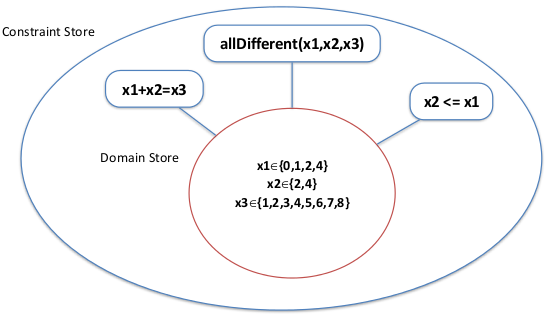
\includegraphics[width=8cm]{fixPoint1}
    & $\Rightarrow$ &
    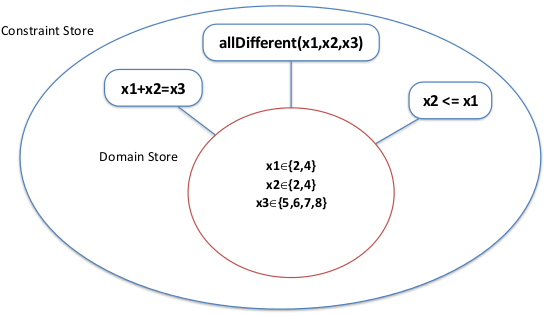
\includegraphics[width=8cm]{fixPoint2}
\end{tabular}


\subsection{Consistency}

\begin{itemize}
    \item A CSP (\textsc{X, D, C}) is $X_{Consistent}$ iff all
        constraints $c \in C$ are $X_{Consistent}$ ($X_{Consistent}$ is
        GAC, BC,\ldots)

    \item A consistency $S_1$ is stronger than a consistency $S_2$ iff all CSP respecting
        $S_1$ also respect $S_2$.

        Note that some consistencies can be \textit{incomparable}

        \begin{center}
            \begin{tabular}{l|c|c|}
                \cline{2-3}
                \multirow{1}{*}{
                    \begin{tikzpicture}
                        \node (0,0) {};
                        \draw[->] (0,1.5) edge node [left]{\rotatebox{90}{Strongest}}
                        (0, 2.5);
                \end{tikzpicture}} 
                &
                \multicolumn{2}{c|}{GAC} \\
                \cline{2-3}
                & Bound consistency & Forward checking \\
                \cline{2-3}
            \end{tabular}
        \end{center}

        This is a tradeoff between \textbf{Speed} and \textbf{Filtering}.

\end{itemize}


\subsubsection{Filtering consistencies}

if $x$ is a domain filtering consistency, a propagator for $x$ will :
from CSP(X, D, X)
\begin{itemize}
    \item return (X, D', C) such that
        \begin{itemize}
            \item D' $\subseteq$ D
            \item (X, D, C) and (X, D', C) equivalent
            \item D' is a nonempty partial solution
            \item (X, D', C) respect $x$
        \end{itemize}
    \item return \textcolor{red}{fail} if no such CSP exists.

        $\to$ not possible to satisfy consistency = unsatisfiable CSP
\end{itemize}

\begin{itemize}
    \item \textbf{Arc consistency} (also called domain consistency):
        every value of every variable participates in a solution of the
        constraint, so all value of variables are \textbf{supported}.

        \begin{tabular}{m{1cm}m{13cm}}
            Note:&
        \begin{itemize}
            \item It's the strongest filtering when considering constraints in isolation.
                \item  GAC $\neq$ satisifability :i A CSP that is GAC may not
        be satisfiable.
        \end{itemize}
        \end{tabular}

        \paragraph{GAC} A constraint $c$ is GAC iff
        \begin{lstlisting}[mathescape]
$\forall x_i \in scope(c)$
    $\forall a_i \in D(x_i)$
        $\exists a_1,..., a_{i-1}, a_{i+1},..., a_r \in D(x_1) \times ... \times D(x_{i-1}) \times D(x_{i+1}) \times ... \times D(x_r)$ such that $(a_1,...,a_r) \in c$
        \end{lstlisting}


    \item \textbf{Bound consistency}: assuming domains are intervals,
        every bound of every variable participates in a solution of the
        constraint.

        \begin{itemize}
            \item GAC can be costly, so a other consistency is to
                only search support for bound.
            \item[$\to$] all valuyes between min and max considered in the domain.
        \end{itemize}


        \paragraph{BC} A constraint $c$ is BC iff
        \begin{lstlisting}[mathescape]
$\forall x_i \in scope(c)$
    $\forall a_i \in \{ \quad min(D(x_i)), max(D(x_i))\quad \}$
        $\exists a_1,..., a_{i-1}, a_{i+1},..., a_r  \in D*(x_1) \times ... \times D*(x_{i-1}) \times D*(x_{i+1}) \times ... \times D*(x_r):$ such that $c(a_1,..., a_r)$

$D*(x_k) = [min(D(x_k)), max(D(x_k))]$
        \end{lstlisting}


    \item \textbf{Forward checking}

        It's like a GAC at the end.

        \paragraph{FC} A constraint $c$ is FC iff
        \begin{lstlisting}[mathescape]
if $\forall x_i \in scope(c):$ $D(x_i) = \{v_i\}$ then $c(v_1, ..., v_r)$
if all but one variable assigned: $c$ is GAC
        \end{lstlisting}
\end{itemize}



\subsection{Global constraints}

\paragraph{Advantage}
\begin{itemize}
    \item Increasing expressivity of CP
    \item Pruning strength because the propagation considered constraint in isolation
        but global constraint is like \textbf{a set of constraint}
    \item Pruning efficiency because no fixed point between small constraints
        but a more flobal reasoning
\end{itemize}

\subsubsection{Decomposition}
A set of constraints $S$ is called the decomposition of $g$ iff :
$$ \forall D(X): sols(X, D(X), \{g\}) = sols(X, D(X), S)$$

\begin{itemize}
    \item GAC pruning equivalent in $S$ and $g$ iff the constraint
        graph of the D is \textbf{acyclic}.

        Otherwise, GAC pruning stronger in global constraint

        \begin{itemize}
            \item GAC on decomposition : supports(s) for each literal on each constraints
                \textbf{separately}
            \item GAC on global constraint: global support(s) for each literal on global constraint
        \end{itemize}


    \item FC pruning stronger in the decomposition
\end{itemize}


\subsubsection{Sum constraint}
\begin{center}
    \texttt{Sum($x_1 + x_2 + ... + x_n$) = K}
\end{center}

\begin{itemize}
    \item \textbf{GAC} for sum constraint is NP-Hard.

        Proof: reduction of subset-sum to GAC for Sum
        \begin{itemize}
            \item subset-sum: a NP-Hard problem for integer set ($S=\{a_1,\cdots, a_r\}$),
                does any non-empty subset of S sums to 0?

            \item reduction to GAC for Sum:
                \begin{lstlisting}[mathescape]
variables  $x_i$ with domains $\{0, a_i\}$
GAC on sum($[x_1,..., x_r], 0$)

if $D(x_i) = \{0\} \forall x_i$ : answer no
else: answer yes
                \end{lstlisting}
        \end{itemize}

       GAC propagator for sum constraint is exponential (unless P=NP).

   \item \textbf{Bound consistency} can be done in $O(n)$

       \begin{lstlisting}[mathescape]
$x_i^{max} = K \sum_{j \neq i} - x_j^{min}$
$x_i^{min} = K \sum_{j \neq i} - x_j^{max}$
       \end{lstlisting}
\end{itemize}

\subsubsection{AllDifferent constraint}
\begin{center}
    \texttt{allDifferent($x_1, x_2,..., x_n$)}
\end{center}

\begin{enumerate}
    \item Build the variable-value graph 

        \begin{tabular}{m{8cm}m{6cm}}
            \begin{itemize}
                \item one node for each variable $x_1,\cdots, x_r$
                \item one node for each value in $\cap D(x_i)$
                \item one edge between $x_i$ and $a$ if $a \in D(x_i)$
                \item[Note:] bipartite graph
            \end{itemize}
            &
            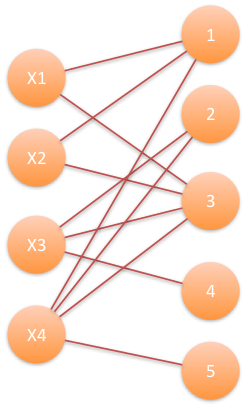
\includegraphics[width=2cm]{variableValue}
        \end{tabular}

    \item There is a solution to allDifferent($x_1, x_2, ..., x_n$)
        if there is a maximum matching of size $n$ in the graph.

        \begin{itemize}
            \item A matching is a \textbf{set of edgges} such that
                no edge share a same node. 
            \item Size matching = \# edges, the maximum size = \#
                variables
        \end{itemize}


        \paragraph{Finding a maximum matching}

        \begin{enumerate}
            \item Start with any matching (e.g. empty matching)
            \item Iteratively improve the matching with \textbf{augmenting path}
                until no more augmenting paths.

                \paragraph{Augmenting path}
                \begin{itemize}
                    \item Edge in M : variables $\to$ values
                    \item Other : values $\to$ variables

                    \item[$\Rightarrow$] An augmenting path is a \textbf{directed path}
                        from a uncovered value to an uncovered variable.
                        Use DSF or BFS
                \end{itemize}

                \begin{figure}[!h]
                    \centering
                    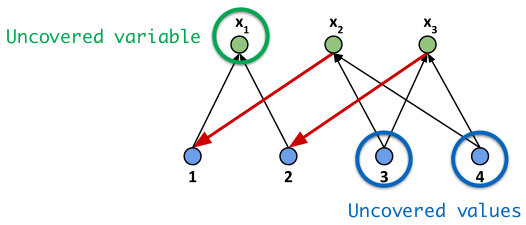
\includegraphics[width=8cm]{augmenting-paths.png}
                    \caption{Augmenting paths}
                \end{figure}

        \end{enumerate}

    \item Remove useless edge by using a \textbf{transformed var-value
        graph} in order to keep edge where there is a directed
        cycle in the transformed graph:
        \begin{itemize}
            \item Alternating path: change value of variable
            \item Alternating cycle: exchange value of variable
        \end{itemize}

        Note that to have the alternate matching, only switch the
        edges in/out.

        \begin{center}
            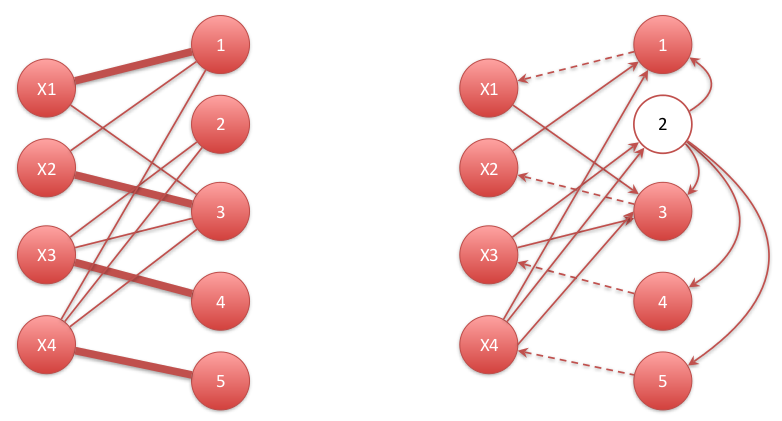
\includegraphics[width=5cm]{transformed}
        \end{center}

        \paragraph{Remove edge}
        Remove all edge $(x, a)$ such that 
        \begin{itemize}
            \item $(x, a)$ is not in the matching 
            \item $a$ and $x$ are in two different Strongly
                Connected Components in the transformed graph because
                there is no directed cycle 
        \end{itemize}

        \paragraph{SCC}
        \begin{enumerate}
            \item Call DFS(G) to compute finishing time $f[u]$ for each vertex


                \begin{tabular}{m{7cm}m{7cm}}
                    \begin{lstlisting}[mathescape]
DFS(V, E):
    // Initialization
    Create global variable Color[1..|V |]
    Create global variable P arent[1..|V |]
    for each node $u \in V$ do
        Color[u] = white
        Parent[u] = Nul
        time = 0

    // Start the search
    for each node $u \in V$ do
        if Color[u] = white then
            Visit(u, V, E)
                \end{lstlisting}
                &
                \begin{lstlisting}[mathescape]
Visit(u, V, E): 
    Color[u] = Grey
    time = time + 1
    d[u] = time

    for $v \in Adj[u]$ do
    // Explore arc (u, v)
        if Color[v] = white then
            Parent[v] = u
            Visit(v, V, E);

    Color[u] = black;
    time = time + 1;
    f[u] = time;
                \end{lstlisting}
                \end{tabular}
            \item compute $G_T$ 
            \item Call DFS(G) but in the main loop of the DFS, consider vertices in order
                of decreasing $f[u]$ as computed in line 1 
            \item Output the vertices of each tree in the DFS forest formed in line 3 as a
                separate SCC
        \end{enumerate}

\end{enumerate}


\subsubsection{Element constraint}

\begin{tabular}{m{6cm}m{6cm}}
    \texttt{Element($c, y$) = x}
    \begin{itemize}
        \item $X = C[Y]$
    \end{itemize}
    &
    \includegraphics[width=6cm]{elements}
\end{tabular}

\subsubsection{Knapsack constraint}
\begin{center}
    \texttt{binaryKnapsack($x=[0, 1, 0], p=[100, 200, 300], w=[1, 5, 3],
    P=400, W=6$)}
\end{center}
Maximize profit while satisfying the capacity.

\subsubsection{BinPacking constraint}
\begin{center}
    \texttt{binPacking($x=[0, 3, 1], w=[1, 5, 3], l=[4, 0, 6]$)}
\end{center}
Placement of weighted items into capacitated bins.

\subsubsection{Hamiltonian circuit constraint}
\begin{center}
    \texttt{circuit($x[CPIntVar]$)}
\end{center}

\begin{tabular}{m{5cm}m{10cm}}
$x(i)$ is visited after $i$
&
    \includegraphics[width=6cm]{hamilto}
\end{tabular}


\subsection{Search}
\begin{itemize}
    \item Recursive search (divide and conquer) with DFS.
        
        The tree is construct during exploration and only the current
        node in memory (DFS). The alternative decisions is memorized.

    \item Branching and variable/value heuristic
        in order to specify for each child nodes
        how to split problem.

        \paragraph{Node expansion}
        Subdivision of a CSP into smaller CSP such that the union of the small CSP
        is equivalent to the original.

\end{itemize}

\subsubsection{Depth First Backtraking search}

\begin{itemize}
    \item Based on:
    \begin{enumerate}
            \item \textbf{stack of sets of decision}
            \item \textbf{stack of restoration states}
        \end{enumerate}
    \item Backtracking restores:
        \begin{enumerate}
            \item Variables/domains
            \item Constraints
            \item Backtracked structures (ex: fistSupport)
        \end{enumerate}
\end{itemize}

\begin{lstlisting}[caption=Depth First backtracking search]
while (! decisionStack.isEmpty) {
    val decisionsOfNode = decisionStack.pop()

    val decision = decisionsOfNode.pop()
    if( decision.hasNext() )
        pushState()

    applyDecision(decision)

    if (!isFailed() ){
        val isExpandable = expand(branching)
        if (! isExpandable) {
            solFound()
            popState()
        }
    } else {
        popState()
    }
}
\end{lstlisting}


\subsubsection{Branching}

\begin{itemize}
    \item A branching strategy is \textbf{completeness}
        if the union of the child CSPs is the parent CSP.

    \item \textbf{Strategy}: 
        \begin{tabular}{l}
            binary labelling ($x_1=a, x_1 \neq a$),\\
            n-ary labelling ($x_1=a, x_1=b, x_1=c, x_1=d$),\\
            domain spliting ($x_1\geq t, x_1 < t$)
        \end{tabular}

    \item \textbf{Variable heuristic}: 
        \begin{tabular}{l}
            Random, lexicographic \\
            Highest number of constraint, variable with unstable
            domain
        \end{tabular}

        \paragraph{First fail principle}: choose first a variable that
        is more likely to fail (Consider the most difficult parts of the
        CSP first).

    \item \textbf{Value heuristic}:
        \begin{tabular}{l}
            Random, lexicographic\\
            Value with minimum pruning, maximum number of solution\\
        \end{tabular}

        \paragraph{Best first principle}: Choose first a value that is
        more likely to succeed
\end{itemize}

\subsubsection{Trailing: restoring state}

\begin{tabular}{m{10cm}m{6cm}}
    In opposition to copying the node in order to perform backtracking,
    trailing only store the \textbf{modification}.

    \begin{itemize}
        \item \textbf{Trail level}
            Trailed operations are marked with an integer which is increase!

        \item \textbf{Restoring} undo all operations with trail level greater than
            desired set the trail level to desired one.
    \end{itemize}

    Sparse set are use to store the domain!
    &
    \includegraphics[width=6cm]{trailing}
\end{tabular}

\paragraph{Sparse set data structure}:


\begin{tabular}{m{7cm}m{1.5cm}}
\begin{itemize}
        \item Composed of two table: $dom$ and $map$
        \item $dom$ is split in two set: value in the domain
            are before \textbf{size} and removed value after.

        \item \textbf{}{Invariant} :
            $$ D = \{dom[i] | 0 \leq i \leq size\}$$
            $$map[v] = i \Leftrightarrow dom[i] = v$$
    \end{itemize}
&
\includegraphics[width=9cm]{sparse.png}
\end{tabular}

\begin{itemize}
    \item \textbf{Checking} if $v$ in the domain: $O(1)$
        \begin{enumerate}
        \item $v \in D \Leftrightarrow map[v] < size$
            \end{enumerate}

    \item \textbf{Removing value} $c$: $O(1)$
        \begin{enumerate}
        \item Exchange value of $map[c]$  and  $map[dom[size-1]$
                \item Decrement $size$ value
            \end{enumerate}

        \item \textbf{Restore removed value}: $0(1)$ thanks to
            ReversibleInteger.

            Note that value are restore in different positions

    \item \textbf{Min/Max} can be added to sparse-set to perform
        efficient BC filtering. 

        When min value are removed, then consider min+1, min+2,...
        until a value in the domain is found (in practive only few
        iterations)

    \item Domain \textbf{iterator} is the only limitation of sparse-set
\end{itemize}



\subsection{Exam}
\begin{itemize}
    \item  Understand how CP works : domain store, fix-point
        algorithm, (reversible) domain implementation.
    \item  Search and First-Fail principle
    \item  Be able to model using element, allDifferent, sum, etc
    \item  Understand Bound-Consistency and Domain
        consistency
    \item  Understand the filtering algorithms for allDifferent, sum,
        etc and be able to design simple filtering algorithms.
\end{itemize}




\section{CP techniques}


\subsection{Scheduling CP}

\begin{center}
    \texttt{cumulative($[s_1,..., s_n], [d_1, ..., d_n], [e_1, ...,
    e_n], [c_1, ..., c_n], C$)}
\end{center}

\begin{itemize}
    \item $\forall_i: s_i + d_i = e_i$
    \item $\forall_t: \sum_{s_i \leq t < e_i} c_i \leq C$
\end{itemize}

\subsubsection{Sweep line algorithm}
It's use to compute the cumulated
profile and check that it does not exceed the capacity.


\begin{enumerate}
    \item \begin{tabular}{m{5cm}m{10cm}}
            \begin{itemize}
                \item One time point for start $(start, +capa)$
                \item One time point for end $(start, -capa)$ 
            \end{itemize}&
                    \includegraphics[width=7cm]{sweepLine}
                \end{tabular}


            \item \begin{tabular}{m{5cm}m{8cm}}
                    \begin{itemize}
                        \item Sort time points
                    \end{itemize}
                    &

                    (0,+7), (0,+10), (10,-7), (10,4), (13,-10), (13,9), (15,4), (18,-9), (22,7), (29,-4), (31,-4), (38,-7)
                \end{tabular}

            \item \begin{tabular}{m{5cm}m{10cm}}
                    \begin{itemize}
                        \item Sweep-line(t) = height of the profile at time $t$.
                    \end{itemize}
                    &
                    \includegraphics[width=7cm]{sweepLine2}
                \end{tabular}

                \begin{lstlisting}[mathescape]
input = eventQueue$[(time,c)]$
t = input.head.time   // Current time of the sweep line
h = 0                 //  current capacity of the sweep line 

while (input.nonEmpty) {
    while (input.nonEmpty && input.head.time == t){
        (time,c) = input.dequeue
        h = h + c
    }
    add (t,h) to the profile
    t = input.top.time
}
            \end{lstlisting}
    \end{enumerate}


\subsubsection{Optimistic Resource Profile}

\begin{tabular}{m{11cm}m{6cm}}
The optimistic resource profile is built based on the
\textbf{mandatory parts} which is the time where the activity will
use the resource whatever it final position.
&
\includegraphics[width=4cm]{mandatory}
\end{tabular}

\begin{itemize}
    \item \textbf{Update minimum start time} at the earliest
        time such that it is not in conflict with the optimistic
        resource profile.

        \paragraph{Time complexity}: $O(n)$ per task since recource
        profile has $O(n)$ intervals. So, $O(n^2)$ overall.
\end{itemize}


\subsection{Large Neighborhood Search}

\begin{tabular}{m{12cm}m{3cm}}
    The diversification is the most weakness of CP for hard COPs.
    The idea of LNS is stuck for too long $\to$ jump in the search space
    by using restart!
    &
    \includegraphics[width=2cm]{LNS}
\end{tabular}

\begin{tabular}{m{2cm}m{11cm}}
    Randomized restart & 
    \begin{itemize}
        \item Use some random decisions in your heuristic (value or variable)
        \item Use a limit on the search (number of backtracks or
            time)
        \item If no feasible solution is found within this limit,
            restart.
    \end{itemize}
\end{tabular}

\subsubsection{LNS work}

\begin{tabular}{m{10cm}m{6cm}}
    \begin{enumerate}

        \item Find a first initial solution, $S*$
        \item Randomly relax $S*$ and re-optimize with search limit

            Relax = fix some variables to their values in $S*$ and CP
            search the other

            \begin{itemize}
                \item A portion of the variables is selected (=\textbf{fragment})
                    and are relaxed to the \textbf{initial domain}
                \item The other variables are frozen to their value in the current solution
                \item A limited CP search \textbf{improving solutions}
            \end{itemize}

        \item Replace $S*$ by the best solution found
    \end{enumerate}

    &
    \includegraphics[width=6cm]{lns.png}
\end{tabular}

\paragraph{Advantages}
\begin{itemize}
    \item Good diversification if fragment well chosen $\Rightarrow$ no
        meta-heuristic needed (tabu,...) because neighborhood is large
        enough
    \item No need to design complex feasible neighborhoods because CP
        is in charge of feasibility

    \item Intensification with CP search and efficient 
        exploration of neighborhoods with CP
    \item Scalability of LS
\end{itemize}


\subsubsection{LNS parameters}
Parameters of LNS :
\begin{itemize}
    \item \textbf{Fragment size} and \textbf{time/backtrack limit}:
       strongly linked parameters because
       \begin{enumerate}
           \item fragment size determines neighborhood size
           \item limit determine the maximal effort to explore
       neighborhood.
       \end{enumerate}

       \paragraph{Note:} a good LNS should never be stopped only by the limit\ldots

       \paragraph{Adaptive versions}:
       \begin{enumerate}
           \item Fix a time/backtrack limit
           \item if neighborhood fully explored $\to$ increase fragment size
           \item else: decrease fragment size
       \end{enumerate}

    \item \textbf{fragment selection} (can be combined).

        Should contain important variables and related variables.

        \begin{itemize}
            \item \begin{tabular}{m{3cm}m{10cm}}
                    Random selection &
                \begin{itemize}
                    \item Surprisingly good
                    \item Generic
                    \item Excellent diversification
                    \item Intensification from CP search
                \end{itemize}
            \end{tabular}

        \item \begin{tabular}{m{3cm}m{10cm}}
                    Specific selection &
                \begin{itemize}
                    \item Only for one problem
                    \item Use knowkedge of the problem to select variables
                    \item Usually randomized to some extend
                \end{itemize}
            \end{tabular}
        \end{itemize}
\end{itemize}

\subsubsection{QAQ}
\begin{tabular}{m{9cm}m{7cm}}
    \begin{lstlisting}
val	cp	=	CPSolver()	
var	w:	Array[Array[Int]]		//weight	matrix	
var	d:	Array[Array[Int]]		//distance	matrix	
val	x	=	N	map	(v	=>	CPIntVar(cp,	0	until	n))	
//matrix	of	variables			representing	the	distances	
val	D	=	Array.tabulate(n,	n)((i,	j)	=>		
									element(d,	x(i),	x(j)))	
val	bestSol	=	Array.fill(n)(0)	
cp.onSolution	{	
	for(i	<-	0	until	n)		
			bestSol(i)	=	x(i).value)	
}	

add(allDifferent(x),	Strong)
minimize(sum(N,	N)((i,	j)	=>	D(i)(j)	*	w(i)(j)))	
search	{	
		binaryFirstFail(x)	
}	start(1)
\end{lstlisting}
&
\begin{lstlisting}[caption=LNS relax]
for (r <- 1 to 300) {
    startSubjectTo(failureLimit = 60) {
        // relax randomly 50% of the variables
        for (i <-N; if rand.nextInt(100) < 50) {
            add(x(i) == bestSol(i))
        }
    }
}
\end{lstlisting}

\begin{center}
    \includegraphics[width=4cm]{QAP}
\end{center}
\end{tabular}

\subsubsection{Vehicle routing}

\textbf{Regret heuristics}: choose the variable with the
greatest difference in cost between the two best values in
its domain. i.e. Measure the impact of not having the best
choice.

\begin{itemize}
    \item Remove the longest arcs in order to have a chance to improve
    \item From routes that are close such that you can relocate customers
\end{itemize}

\subsubsection{Cutting stock}

    \begin{itemize}
        \item $X_i \in N$: the number of planks with configuration $i$
            produced where a configuration is a possible assignment of
            roll type to a plank.

        \item Configuration $i: [a_{1i}, a_{2i}, ..., a_{ni}]$ where
            $a_{ji}$ is the number of roll type $j$ (width $w_j$) in
            configuration $i$.

            Note that there is a exponential number of
            configurations
    \end{itemize}

\begin{tabular}{m{5cm}cm{5cm}}
    \begin{eqnarray*}
        \textrm{minimize } & \sum_i X_i \\
        \textrm{Subject to } & \sum_i X_i a_{ji} \geq b_j
        \forall_j\\
        & x_i \geq 0
    \end{eqnarray*}
    & $\Leftrightarrow$ Strong LP duality $\Leftrightarrow$ & 
    \begin{eqnarray*}
        \textrm{minimize } & \sum_i b_i Y_i \\
        \textrm{Subject to } & \sum_i Y_i a_{ji} \geq 1
        \forall_j \\
        & Y_i \geq 0
    \end{eqnarray*}
\end{tabular}

\begin{center}
\includegraphics[width=13cm]{column}
\end{center}

\begin{itemize}
    \item Find a configuration $[\alpha_1, ..., \alpha_n]$ such that:
        $$1 - \sum_i \alpha_i Y_i < 0$$
        If there isn't such configuration, we prove the optimality of the
        linear program

    \item[$\Rightarrow$] Pricing is a Knapsack problem:
        \begin{eqnarray*}
            \textrm{Maximize } & \sum_i \alpha_i Y_i\\
            \textrm{Such that } & \sum_i \alpha_i w_i \leq W
        \end{eqnarray*}

        Note that $\alpha_i$ are the variables and $Y_i$ are constants
        given as by product of the simplex
\end{itemize}

\begin{center}
\includegraphics[width=13cm]{column2}
\end{center}


\paragraph{Column generation}
\begin{enumerate}
    \item Start with a limited number of patterns
    \item Solve the master problem 
    \item  Generate a new column (with CP/LS/B\&B/...) with negative reduced cost, if
        not possible stop
\end{enumerate}

\paragraph{Column generation by SINFO22}
\begin{enumerate}
    \item Generate a few valid columns to start with

    \item  Solve the dual problem using simplex to get optimal $Y_i$ directly,
        or solve the primal problem to get optimal $X_i$ which you can then
        use to compute the optimal $Y_i$ using complementarity conditions.
        Both these techniques were not seen in class, although if you know
        the dual problem, applying simplex on it is just as easy as applying
        it on the primal.

    \item  Once you have the $Y_i$, you need to find 'a' such that $1 - \sum_i
        Y_i * a_i$ is negative. If you find such an $a$, you can include as a
        new pattern in your simplex tableau and since the reduced cost is
        negative, it will help reduce the objective. You could use any 'a'
        that produces negative reduced cost, but it's better to pick the
        most negative one directly. Since minimizing $1-\sum_i Y_i*a_i$ is
        equivalent to maximising $\sum_i Y_i * a_i$, you will solve the
        maximization problem instead. You cannot pick any 'a' because it
        still need to be a valid pattern (it must fit on a plank...), so you
        have to add the $\sum_i a_i <= L$ constraint where L is the length of
        the plank.

    \item  Now you have a new pattern, and you can include it in your
        simplex. You then iterate your simplex until you find an optimal
        solutions that uses only the few columns that you included. When you
        reach the optimum, you don't know if it's the real optimum of the
        problem because you're only looking at solutions using a few
        columns. You need to restart at step 3 and keep adding columns until
        step 3 can't find a column with negative reduced cost (the
        maximization procedure will give a value <= 1. When that's the case,
        you know you're done).
\end{enumerate}

\paragraph{Hybridization}

Is it because, on one hand, we have a linear program for minimizing an
objective with a limited set of column, and on the other hand, we have
another algorithm (e.g. Branch \& Bound, Local search, LNS,...) for
generating a column with the smallest negative reduced cost (if such a
column exists) ?
So we have an hybridization between the linear program and the other
algo ?


\subsection{Exam}
\begin{itemize}
    \item  Be able to explain the sweep line algorithm and be
        able to execute it to compute a resource profile
    \item  Understand how to use the (optimistic) resource profile
        to filter the domain of start/end variables
    \item  Explain what is LNS, what is the advantage of using it
        over pure CP, what do we loose (proof of optimality)?
    \item  Be able to suggest LNS relaxation for a problem
    \item  Explain what is column generation. In what sense does
        it allow hybridization
\end{itemize}





\section{Derivative free optimization}

It's not always possible to use derivative in order to optimize a
fonction with a continuous domain because:
\begin{enumerate}
    \item  The gradient is not computable
    \item  We dont know the objective function
    \item  The gradient is to expensive to compute
    \item  We don't know how to compute the gradient
\end{enumerate}

In this case, we can use \textbf{Derivative free optimization}.
We dont know the objective function but we have comparison function that allows us to compare solutions.


\subsection{Background}

\subsubsection{Single-objective Optimization problem}
\begin{tabular}{m{6cm}m{6cm}}
    \begin{eqnarray*}
        \textrm{Optimize } & f(X)\\
        \textrm{subject to } & X \in \Omega\\
    \end{eqnarray*}
    &
    where $ \begin{cases}
        X = (x_1, ..., x_n)\\
        f: \Omega \rightarrow \mathbb{R}\\
        \Omega \subseteq \mathbb{R}^n
    \end{cases}$
\end{tabular}

\subsubsection{Feasible Region}

Only consider $\Omega \subseteq \mathbb{R}^n$ which define hyper-volume:
$$\forall_i \in 1,..., n: \Omega_i = [l_i, u_i]$$ 
where $l_i, u_i \in \mathbb{R} and l_i \leq u_i$

\subsubsection{Comparison function}
$$cmp(x_1, x_2) : \Omega^2 \rightarrow \mathbb{B}$$

\paragraph{Example}
\begin{itemize}
    \item Classical minimization: $(x_1, x_2) \Rightarrow f(x_1)\leq
        f(x_2)$
    \item Classical maximization: $(x_1, x_2) \Rightarrow f(x_1)\geq
        f(x_2)$
    \item Probabilistic minimization: $(x_1, x_2) \Rightarrow E[f(x_1)]\geq
        E[f(x_2)]$
    \item ...
\end{itemize}

\subsection{Grid Search}

As the domain is continuous and we can't compare every point:

\begin{tabular}{m{10cm}m{7cm}}
\begin{enumerate}
    \item Cut each dimension of the domain $\Omega$ in m
    \item Evaluate each one of these combination 
    \item Output the minimum

    \item[$\Rightarrow$]  We will always have $m^n$ evaluation,
        because we have $n$ dimensions that
we cut in $m$ parts.
\end{enumerate}
&
\includegraphics[width=4.5cm]{grid}
\end{tabular}

\subsubsection{Iteratively}
\begin{itemize}
    \item Perform a grid search for the domain $\Omega$ 
    \item Around the min point found define a new smaller domain
        $\Omega$ 
    \item[$\Rightarrow$] So if we do i iterations we will have $i *
        m^n$ evaluations for the objective.
\end{itemize}

\subsection{Directional Direct Search}

\begin{tabular}{m{12cm}m{3cm}}
The global idea is to \textbf{test a sample of points} in specified
directions around the iterate.
If a point is better, select it as next iterate.
&
\includegraphics[width=2cm]{DDS}
\end{tabular}

\subsubsection{Step}

\begin{enumerate}
    \item \textbf{Poll step}: Test $N$ points in specified directions
        around iterate and stop when better (with our comparison
        function) point found.

        \begin{itemize}

            \item \textbf{Directions and bases}
                We define a set $D$ of positive bases used to evaluate new
                points (directions):
                $$D = [l, -l] = [e_1,..., e_n, -e_1,..., -e_n]$$
                where the $e_i (1 < i < n)$ are unit vector ($||e_i|| = 1$)

            \item \textbf{Build new point} around the iterate $x$:
                $$x_{new} = x+\alpha*d \quad \textrm{where } d \in D$$
        \end{itemize}

        \paragraph{Example} For a 3D space,
        $$D = [l, -l] = [e_1, e_2, e_3, -e_1, -e_2, -e_3] \quad
        \textrm{where} \quad \begin{cases}
            e_1 = (1,0,0) \\
            e_2 = (0,1,0)\\
            e_3 = (0,0,1)\\
        \end{cases} $$
        $$\textrm{Suppose} \quad \begin{cases} 
            x = (40, 42, 42)\\
            d = (1, 0, 0)\\
            \alpha =2
        \end{cases} \quad           
        x_{new}  = (40, 42, 42) + 2 * (1, 0, 0) = (42, 42, 42)$$


    \item \textbf{Mesh parameter update}: Update or maintain the step
        size parameter, $\alpha_k$ in order to converge faster.

        \begin{enumerate}
            \item Iteration declared successful: increase $\alpha_k$ to
                perform greater step
                $$\alpha_{k+1} = \gamma \alpha_k \quad \textrm{with}\quad \gamma > 1$$

            \item Iteration declared unsuccessful: decrease $\alpha_k$ to
                converge to an optimum
                $$\alpha_{k+1} = \beta \alpha_k \quad \textrm{with}\quad
                0 < \beta < 1$$
            \end{enumerate}
\end{enumerate}

\subsubsection{Denis-Wood Coutours}

\begin{tabular}{m{12cm}m{5cm}}
No convergence if Denis-Wood contours appears in objective
function
&
\includegraphics[width=2cm]{contour}
\end{tabular}

\begin{tabular}{m{3cm}m{10cm}}
    $\Rightarrow$ Two solutions:&
\begin{enumerate}
    \item Rotate the bases after $N$ unsuccessful iterations
    \item Run DDS $N$ times with $N$ different set of bases.
    \end{enumerate}
    \end{tabular}

\subsubsection{One iteration complexity}
\begin{itemize}
    \item Worst case: $Nb_{evals} = 2b = 0(b)$ where $b$ is the number
        of bases used
    \item Best case: $Nb_{evals} = 1 = \Omega(1)$
\end{itemize}


\subsection{The Nelder-Mead Algorithm}

The global idea is to build a structure of points and replace the worst
point at each iteration.

\subsubsection{Simplex}
\begin{tabular}{m{12cm}m{3cm}}
    \begin{itemize}
        \item The structure of point is a polyhedron of dimension $n+1$
            (abusively called simplex)

    \item The simplex structure $Y$ is a set of $n+1$ vertices where $n$ is the
dimension of the search space defined as follows:
$$Y = \{y^0,y^1,...,y^n\}$$

\item The vertice $y^0$ is a better solution than the vertice $y^1$ which is a better solution that then vertice $y^2$ ....
        \end{itemize}
&
\includegraphics[width=3cm]{polyhedron}
\end{tabular}

\subsubsection{Operations on the simplex}
At each iteration, replace the worst point by performing one of the
following actions:
\begin{enumerate}
    \item \begin{tabular}{m{11cm}m{3cm}}
            \textbf{Reflection} if $f^0 \leq f^r < f^{n-1}$ : Replace $y^n$ by $y^r$

            $$Nb_{evals} = 1 = \Theta(1)$$

            It's implies that $f^r$ which replace the worst point ($y^n$) are better than
            the previous worst point ($y^{n-1}$)
            & 
            \includegraphics[width=5cm]{reflection}
        \end{tabular}

    \item \begin{tabular}{m{11cm}m{3cm}}
            \textbf{Expansion} if $f^r < f^0$ : 
            \begin{itemize}
                \item If $f^e \leq f^r$ replace $y^n$ by $y^e$
                \item else replace $y^n$ by $y^r$
            \end{itemize}

            $$Nb_{evals} = 2 = \Theta(1)$$

            If the $y^r$ are the better point between all $y^i$, try to
            expand him more to have a still better point
            & 
            \includegraphics[width=5cm]{expansion}
        \end{tabular}

    \item \begin{tabular}{m{11cm}m{3cm}}
            \textbf{Contraction} if $f^r \geq f^{n-1}$ : 
            \begin{itemize}
                \item If $f^r < f^n$ replace $y^n$ by $y^{oc}$ (outside)
                \item else replace $y^n$ by $y^{ic}$ (inside)
            \end{itemize}

            $$Nb_{evals} = 2 = \Theta(1)$$

            If $y^r$ is a worst point than $y^{n-1}$ then contract him 
            toward other point and take outside if he is still better
            than $y^n$, otherwise inside.
            & 
            \includegraphics[width=5cm]{contraction}
        \end{tabular}

    \item \begin{tabular}{m{11cm}m{3cm}}
            \textbf{Shrink} if no amelioration by doing thos 

            $$Nb_{evals} = n+2 = \Theta(n) \quad \textrm{with n the
            dimension of search space}$$ 

            If no other work, bring all point closer to the best one
            $y^0$
            & 
            \includegraphics[width=4cm]{shrink}
        \end{tabular}
\end{enumerate}


\subsection{Multi-Directional Search}

Globally, it's the same point structure than in Nelder-Mead.
\begin{itemize}
    \item Perform operations on all but one vertices of the simplex around
        the best vertex.

    \item The structure of point is a polyhedron of dimension n + 1 (The
        simplex of Nelder-Mead).
\end{itemize}

\subsubsection{Operations on the simplex}
$$\textrm{Evaluate }: f^r = min \{ f(y_i^r) | i=1,...,n\}$$
\begin{enumerate}
        %TODO
    \item \begin{tabular}{m{11cm}m{3cm}}
            \textbf{Rotation } :\begin{itemize}
                \item if $f^r$ < $f^0$ -> expansion
\item else -> contract simplex 
    \end{itemize}

            $$Nb_{evals} = n = \Theta(n) \quad \textrm{with n the
            dimension of search space}$$ 
            & 
            \includegraphics[width=4cm]{rotate}
        \end{tabular}

    \item \begin{tabular}{m{11cm}m{3cm}}
            \textbf{Expansion } 
            \begin{itemize}
\item if $f^e$ < $f^r$ -> The new simplex is the expanded simplex
\item else -> cThe new simplex is the rotated simplex 
    \end{itemize}

            $$Nb_{evals} = 2n = \Theta(n) \quad \textrm{with n the
            dimension of search space}$$ 
            & 
            \includegraphics[width=4cm]{expand}
        \end{tabular}

    \item \begin{tabular}{m{11cm}m{3cm}}
            \textbf{Shrink} if no amelioration by doing thos 

            $$Nb_{evals} = 2n = \Theta(n) \quad \textrm{with n the
            dimension of search space}$$ 
            & 
            \includegraphics[width=3cm]{shrink}
        \end{tabular}
\end{enumerate}



\subsection{Smart Random Algorithms}
\begin{itemize}
    \item Problem: Algorithm might convert to local minimum.
    \item Solution:  Restart from different points
\end{itemize}

\subsubsection{Random restarts}
\begin{itemize}
    \item Run $N$ times the algorithm such as:
        \begin{enumerate}
            \item For each run the algorithm begins from a random starting
                point
            \item Random starting points following a uniform distribution
            \item Return the best result obtained over the N runs
        \end{enumerate}

    \item [$\Rightarrow $] With $N \rightarrow \infty $ we will
        eventually converge to a global optimum byt this take too much
        computation
\end{itemize}

\subsubsection{Halton sequence}

To perform better random sequence, we need to \textbf{reduce gaps
between point} which is the job of Halton sequence.

\begin{itemize}
    \item \textbf{Build 1D Halton sequence}
        \begin{enumerate}
            \item Choose a base (integer) 
            \item Successively decompose [0, 1]
                in subintervals according to the base.
        \end{enumerate}

        $$\textrm{Example base 2: } \frac{1}{2},
        \frac{1}{4},\frac{3}{4}, \frac{1}{8}, \frac{5}{8},
        \frac{3}{8}, \frac{7}{8}, ...$$

    \item \textbf{Build Multi-D Halton sequence}
        \begin{enumerate}
            \item Build $n$ 1D sequence with $n$ different bases (prime
                two by two)
            \item Mix them to build point
        \end{enumerate}


        $$\textrm{Example : } \Bigg[(\frac{1}{2}, \frac{1}{3}),
            (\frac{1}{4}, \frac{2}{3}), (\frac{3}{4}, \frac{1}{9}), (\frac{1}{8},
        \frac{4}{9}),(\frac{5}{8}, \frac{7}{9})\Bigg]    \quad
        \textrm{from } \quad
        \begin{cases}
            \frac{1}{2}, \frac{1}{4},\frac{3}{4}, \frac{1}{8}, \frac{5}{8}\\
            \frac{1}{3}, \frac{2}{3},\frac{1}{9}, \frac{4}{9}, \frac{7}{9}
        \end{cases}$$

\end{itemize}


\paragraph{Problem} With higher prime sequence, there is a correlation
problem.

\begin{itemize}
    \item[$\Rightarrow$] The solution is to \textbf{shuffle} all 1D sequences before
        mix them to build points 
\end{itemize}



\section{Optimization}

\subsection{Bi-objective optimization}

Assume that you want to minimize two objectives (ex: risk and cost).
Objective are not always comparable often conflicting.

\begin{itemize}
    \item \textbf{Lexicographic optimization}: You consider that one of
        the objective is much more important than the other one.

        For example, in vehicle routing, we prefer (6trucks, 500km) rather
        than (7trucks, 250km) because driver are costly than kilometers.

        \begin{enumerate}
            \item Minimize the first objective and found $T*$ the number
                of trucks

                \textit{In practive done with column generation for
                instance}
            \item Minize the second objective according to 
                the first minimization, so number of trucks $\leq T*$

                \textit{In practice, use local search to improve
                solution generated by column generation}
        \end{enumerate}

    \item \textbf{Weighted objective}: Monetize each objective. 
        The problem is that you don’t always have these costs,
        and you may want to generate \textit{candidate} solutions
        event before these costs are known.

    \item \textbf{Dominance}
        \begin{center}
            \includegraphics[width=11cm]{dominance}
        \end{center}

\end{itemize}


\subsubsection{Pareto set (efficient set)}
A solution is efficient iff it is not dominated by any
satisfiable solution. The goal if to discover the \textbf{Pareto set}
without considering every possibles feasible solutions.

\begin{itemize}
    \item \textbf{Weighted Sum}:  Find point on the \textbf{convex hull}
        of the pareto front for the bi-objective 

        \begin{lstlisting}[mathescape]
step = 0.1
$\alpha = 0$
setPareto = $\emptyset$
while $\alpha < 1$ do
    minimize $\alpha * obj_1 + (1-\alpha) * obj_2$
    setPareto = setPareto $\cup (obj_1*, obj_2*)$
    $\alpha +=$ step
    \end{lstlisting}

    \begin{tabular}{m{10cm}m{6cm}}
        \includegraphics[width=10cm]{weighted}
        &
        \begin{itemize}
            \item As only the convex hull of the pareto front can be
                discover, some points (red) can be miss in the concave parts
        \end{itemize}
    \end{tabular}

    $\Rightarrow$ \begin{tabular}{l}
        Only discover subset of points on the convex hull\\
        Can be generalized to more than two objective\\
        $\alpha$ not easy to find (too small $\alpha$ will rediscover
        the same solution several times)
        \end{tabular}

    \item \textbf{Epsilon constraint}: Find pareto front for the
        bi-objective

        \begin{lstlisting}[mathescape]
$\epsilon$ = 0.1
setPareto = $\emptyset$
$o_2 = \infty$
ok = true
while ok do
    ok = false
    minimize $obj_1$ subject to $obj_2 \leq o_2* - \epsilon$
    if solution found then
        ok = true
        setPareto = setPareto $\cup (obj_1*, obj_2*)$
        $o_2 = obj_2*$
    \end{lstlisting}

    \begin{center}
        \includegraphics[width=10cm]{epsilon}
    \end{center}

    $\Rightarrow$ \begin{tabular}{l}
        Find the real pareto set\\
        Only for two objective\\
        $\epsilon$ should not be too small, but in practice it does not
        regenerate two times the same solution
    \end{tabular}

\end{itemize}

\subsubsection{Pareto set properties}
Sometimes it is too costly to compute the exact Pareto front. We
can use heuristic methods to approximate it (local search).

\begin{itemize}
    \item \textbf{Hyper-volume and diversified} 
        \begin{center}
            \includegraphics[width=8cm]{paretoProperties}
        \end{center}

    \item \textbf{Purity measure}
\end{itemize}


\subsection{Benchmarking optimization}

\begin{itemize}
    \item \textbf{Arithmetic mean of normalized results}: 
        \begin{enumerate}
            \item Assume that for each instance, we have
                measured the time required to reach optimality.
            \item Normalize them and check the result
                \begin{center}
                    \includegraphics[width=11cm]{arithmetic}
                \end{center}

                Note, use \textbf{geometric mean} to have right 
                aggregate results (instead of average) : $\bigg(\prod_{n=1}^k
                x_n\bigg)^{\frac{1}{k}}$

        \end{enumerate}


    \item \textbf{Performance profiles}: $n_p$ instances for which we record various
        things for $n_s$ solvers. $t_{p,s}$ is th e time to solve $p$ by
        $s$.
        \begin{eqnarray*}
            \textrm{Performance ratio: } & \quad r_{p,s} &=
            \frac{t_{p,s}}{min\{t_{p,s}: s\in S\}}\\
            \textrm{Performance profile: } & \quad \rho_s(\tau)&=
    \frac{1}{n_p} \quad size \quad \{\quad p \in P: r_{p,s} < \tau\quad \}
    \end{eqnarray*}

    The performance profile is the probability for solver $s \in S$ to
    have a performance ratio within a factor $\tau$ of the best possible
    ratio. It's a cumulative distribution function of a performance
    metric.

    $\Rightarrow$ solvers with large probability $\rho_s(\tau)$ are to
    be preferred.
                \begin{center}
                    \includegraphics[width=11cm]{profiles}
                \end{center}



\end{itemize}


\subsection{Exam}
\begin{itemize}
    \item Multi-criteria optimization: Understand the three
        methods (lexicographic, weighted sum, Pareto-set).
    \item  Understand the dominance relations between
        solutions.
    \item  Be able to explain how to find a Pareto-set for a bi-
        objective problem.
    \item  Be able to explain why a weighted-sum method is not
        guaranteed to find the true Pareto-set.
    \item  Be able to build a performance profile and analyze it
\end{itemize}


\subsection{Discrete event simulation}
%TODO




\end{document}
